%%%%%%%%%%%%%%%%%%%%%%%%%%%%%%%%%%%%%%%%%%%%%%%%%%%%%%%%%%%%%%%%%%%%%%%%%%%%%%%%%%%%%%%%%
% 
% Document class for MEEC@DEE@ISEP dissertations, by Vitor M. R. Cunha - v1.4, Mar 2024
% Suggestions and comments are welcomed (vrc at isep dot ipp dot pt).
%
% Template provided as is, NO SUPPORT will be given.
% NO questions related to LaTeX will be answered, go to
% https://ftp.eq.uc.pt/software/TeX/info/lshort/english/lshort.pdf, or search the web.
%
% The DEE document class uses the LaTeX book base class, the original work credits are
% in the document class file.
%
% Overleaf template direct link:
% https://www.overleaf.com/latex/templates/isep-meec-msc-thesis-slash-dissertation-latex-template/zdyypsqypqnm
% or go to https://www.overleaf.com/gallery/, and search for: ISEP MEEC
%
%%%%%%%%%%%%%%%%%%%%%%%%%%%%%%%%%% MAIN SETTINGS %%%%%%%%%%%%%%%%%%%%%%%%%%%%%%%%%%%%%%%%

\documentclass[
MEECAS,			% Use this option to select your DEE degree, options: MEECAS, MEECSA, MEECPI, MEECTE
portuguese,		% Select document language, options: portuguese or english
%draft,			% Uncomment for draft mode (no pictures, no links, overfull hboxes) 
]{DEEclass}

% Use the 'preamble.tex' file (root folder) do add packages and macros. Keep your main.tex file clean.

% FYI, the following packages are preloaded with the document class:
% longtable, xcolor, graphicx, booktabs, caption, csquotes, hyperref,
% calc, listings, datetime2, siunitx, geometry, enumitem

%%%%%%%%%%%%%%%%%%%%%%%%%%%%%%%%%%%%%%%%%%%%%%%%%%%%%%%%%% extra packages
\usepackage{amsmath}		% the main package in the AMS-LATEX distribution
\usepackage{amsfonts}		% extended set of fonts for use in mathematics
\usepackage{amssymb}		% adds new symbols to be used in math mode
\usepackage{mathrsfs}		% math fonts, e.g., Laplace
\usepackage{float}			% provides the H float modifier option
\usepackage{multirow}		% tables \multirow command
\usepackage{subcaption}		% enables subfigures
\usepackage{lscape}			% for landscape mode
\usepackage{verbatim}		% new verbatim environment, \begin{comment}...\end{comment}, \verbatiminput
%\usepackage{pgfgantt}		% for Gantt charts, see https://ctan.org/pkg/pgfgantt

%add extra packages if needed here

%%%%%%%%%%%%%%%%%%%%%%%%%%%%%%%%%%%%%%%%%%%%%%%%%%%%%%%%%% temp packages
\usepackage{lipsum}						% for fake text
%\usepackage[textsize=tiny]{todonotes}   % enable To-do notes, use the option "disable" to hide all notes, usage \todo{}

%\usepackage{draftwatermark}			% prints a watermark overlay, uncomment if needed
%\SetWatermarkText{**DRAFT**}
%\SetWatermarkScale{1}
%\SetWatermarkColor[gray]{0.8}

%%%%%%%%%%%%%%%%%%%%%%%%%%%%%%%%%%%%%%%%%%%%%%%%%%%%%%%%%% settings
\AtBeginDocument{					% Rendered PDF metadata:
\hypersetup{pdftitle=\ttitle} 		% Sets the PDF title to your dissertation title
\hypersetup{pdfauthor=\authorname} 	% Sets the PDF author to your name
}

%%%%%%%%%%%%%%%%%%%%%%%%%%%%%%%%%%%%%%%%%%%%%%%%%%%%%%%%%% user macros

%....









% Pacotes adicionais necessários às tabelas, equações e diagrama do conteúdo.
% Nenhuma redefinição da apresentação da classe original.
\usepackage{array,tabularx,tikz}
\usetikzlibrary{arrows.meta,positioning,calc}
\newcolumntype{Y}{>{\raggedright\arraybackslash}X}
\newcommand{\grau}[1]{#1^{\circ}}
\newcommand{\sat}{\operatorname{sat}}
\newcommand{\diag}{\operatorname{diag}}
\newcommand{\R}{\mathbf{R}}
\newcommand{\vet}[1]{\boldsymbol{#1}}
\newcommand{\fonte}{\par\smallskip\footnotesize Fonte: elaboração própria.}

% Marcador para partes por completar (aparece a vermelho no PDF)
\newcommand{\acompletar}[1]{\textcolor{red}{\textit{[A completar: #1]}}}
\usetikzlibrary{shapes.geometric,fit,backgrounds}
\usepackage[european]{circuitikz}
		 

%%%%%%%%%%%%%%%%%%%%%%%%%%%%% DISSERTATION INFORMATION %%%%%%%%%%%%%%%%%%%%%%%%%%%%%%%%%%

\thesistitle{Plataforma estabilizada de dois eixos} % Your dissertation title

\subdate{Outubro, 2026} % Uncomment for a static submission date, or leave it as a comment for automatic date 

\author{Gonçalo Gonçalves e Tomas Pissarra}	% Your name
\studentone{Gonçalo Gonçalves}{1211710}{1211710@isep.ipp.pt}
\studenttwo{Tomas Pissarra}{1221334}{1221334@isep.ipp.pt}

%\advisor{Nome do Orientador}{xxx@isep.ipp.pt}	% Your advisor's name and email
%\coadvisor{Nome do Coorientador}{xxx@isep.ipp.pt}	% Your co-advisor's name and email, comment this line if not needed
%\company{Nome da Empresa, Lda.}	% The company name where you developed your work, comment this line if not needed
%\supervisor{Nome do Orientador da Empresa}{xxx@emailaddress.com}	% Your supervisor's name, comment this line if not needed

%%%%%%%%%%%%%%%%%%%%%%%%%%%%% USER DEFINED LISTS %%%%%%%%%%%%%%%%%%%%%%%%%%%%%%%%%%%%%%%%
\makeglossaries						% Consider the following files in the 'front' folder:
%\input{front/0_glossary}			% Edit to define your glossary entries list
% Lista de acrónimos
% No texto: \gls{chave} (1.ª vez escreve por extenso, depois só a sigla)
% Em tabelas, legendas e títulos: \acrshort{chave}
\newacronym{adc}{ADC}{\textit{Analog-to-Digital Converter}}
\newacronym{adrc}{ADRC}{\textit{Active Disturbance Rejection Control}}
\newacronym{ble}{BLE}{\textit{Bluetooth Low Energy}}
\newacronym{bldc}{BLDC}{\textit{Brushless Direct Current}}
\newacronym{ce}{CE}{Conformidade Europeia}
\newacronym{dc}{DC}{\textit{Direct Current}}
\newacronym{edr}{EDR}{\textit{Enhanced Data Rate}}
\newacronym{ekf}{EKF}{\textit{Extended Kalman Filter}}
\newacronym{esc}{ESC}{\textit{Electronic Speed Controller}}
\newacronym{hal}{HAL}{\textit{Hardware Abstraction Layer}}
\newacronym{i2c}{I\textsuperscript{2}C}{\textit{Inter-Integrated Circuit}}
\newacronym{imu}{IMU}{\textit{Inertial Measurement Unit}}
\newacronym{led}{LED}{\textit{Light-Emitting Diode}}
\newacronym{lqg}{LQG}{\textit{Linear Quadratic Gaussian}}
\newacronym{lqr}{LQR}{\textit{Linear Quadratic Regulator}}
\newacronym{mems}{MEMS}{\textit{Micro-Electro-Mechanical Systems}}
\newacronym{mpc}{MPC}{\textit{Model Predictive Control}}
\newacronym{pid}{PID}{controlador proporcional, integral e derivativo}
\newacronym{pwm}{PWM}{\textit{Pulse Width Modulation}}
\newacronym{red}{RED}{\textit{Radio Equipment Directive}}
\newacronym{reee}{REEE}{resíduos de equipamentos elétricos e eletrónicos}
\newacronym{rohs}{RoHS}{\textit{Restriction of Hazardous Substances}}
\newacronym{spi}{SPI}{\textit{Serial Peripheral Interface}}
\newacronym{spp}{SPP}{\textit{Serial Port Profile}}
\newacronym{sram}{SRAM}{\textit{Static Random-Access Memory}}
\newacronym{uart}{UART}{\textit{Universal Asynchronous Receiver-Transmitter}}
\newacronym{ubec}{UBEC}{\textit{Universal Battery Elimination Circuit}}
\newacronym{ue}{UE}{União Europeia}

%\input{front/0_symbols}				% Edit to define your symbols entries list

%%%%%%%%%%%%%%%%%%%%%%%%%%%%%%%%%%%%%%%%%%%%%%%%%%%%%%%%%%%%%%%%%%%%%%%%%%%%%%%%%%%%%%%%%
\begin{document}
\frontmatter

%----------------------------------------------------------------------------------------
%	TITLE PAGES
%----------------------------------------------------------------------------------------
\pagestyle{plain} % Default to the plain heading style until the thesis style is called for the body content
\printcoverpage
\printaftercoverpage
\cleardoublepage















%%%%%%%%%%%%%%%%%%%%%%%%%%%%%%%%%%% FRONTMATTER %%%%%%%%%%%%%%%%%%%%%%%%%%%%%%%%%%%%%%%%%
% Consider the following front matter sections provided as separate files in the 'front' folder.
% Comment the lines regarding the sections you will not use, or edit the file contents as needed

%\include{front/1_dedicatory}		% Edit if you want to dedicate your work to someone, or comment this line if not used
%\include{front/2_acknowledgements}	% Edit to add the due acknowledgements, or comment this line if not used
%\begin{abstract}
Este estado da arte analisa uma plataforma com dois graus de liberdade, destinada a reproduzir a inclinação de um telemóvel e a manter-se horizontal quando a sua base é perturbada em \textit{pitch} e \textit{roll}. A revisão centra-se na relação entre o problema de controlo, as grandezas que podem ser medidas e a interface efetivamente disponibilizada pelos atuadores.

São discutidos a fusão de sensores inerciais, a identificação dinâmica, o PID com mecanismos de saturação, o controlo em cascata, a compensação antecipativa, o controlo por realimentação de estado, o controlo preditivo, os observadores de perturbação e os métodos robustos, adaptativos e de lógica difusa. A comparação é apoiada por trabalhos científicos sobre plataformas estabilizadas e sistemas de nivelamento, distinguindo resultados experimentais de resultados de simulação.

A análise de hardware abrange a NUCLEO-F767ZI prevista para o projeto, sensores inerciais, servos convencionais e inteligentes, motores com encoder, comunicação sem fios, alimentação e construção mecânica. Propõe-se uma arquitetura inicial com realimentação da atitude da plataforma, PI/PID externo e, quando exista uma segunda IMU, compensação do movimento da base. A evolução para métodos mais complexos fica dependente da identificação do sistema e de melhorias demonstradas por ensaios repetíveis.

\vspace*{10mm}\noindent\textbf{\keywordslabel}: plataforma estabilizada; pitch e roll; PID; rejeição de perturbações; IMU; servomotor; controlo embarcado.

\medskip
\textbf{Âmbito documental.} Revisão narrativa orientada ao projeto, com pesquisa atualizada em 8 de outubro de 2026. As escolhas propostas e os exemplos de cálculo são análise de engenharia, não resultados experimentais do protótipo. O modelo exato da IMU, dos servos e a geometria final ainda carecem de confirmação.

\end{abstract}
\begin{secondlangabstract}
This state-of-the-art review examines a two-degree-of-freedom platform intended to reproduce the inclination of a smartphone and remain horizontal when its base is disturbed in pitch and roll. The review focuses on the relationship between the control problem, the quantities that can be measured, and the interfaces actually provided by the actuators.

The discussion covers inertial sensor fusion, dynamic identification, PID with saturation handling, cascade control, feedforward compensation, state feedback, predictive control, disturbance observers, and robust, adaptive and fuzzy methods. The comparison draws on scientific studies of stabilized platforms and leveling systems, distinguishing experimental evidence from simulation results.

The hardware analysis addresses the planned NUCLEO-F767ZI board, inertial sensors, conventional and smart servos, motors with encoders, wireless communication, power supply and mechanical construction. An initial architecture is proposed using platform attitude feedback, external PI/PID control and, when a second IMU is available, base-motion compensation. Progression to more complex methods depends on system identification and improvements demonstrated through repeatable tests.

\vspace*{10mm}
\noindent\textbf{\keywordslabel}: stabilized platform; pitch and roll; PID; disturbance rejection; IMU; servomotor; embedded control.

\medskip
\textbf{Document scope.} Project-oriented narrative review, with research updated on 8 October 2026. Proposed choices and numerical examples are engineering analysis, not experimental results from the prototype. The exact IMU and servo models and the final geometry remain to be confirmed.
\end{secondlangabstract}
			% Edit the file to write the dissertation Abstract. Two languages are always required.
%----------------------------------------------------------------------------------------
%	FONTMATTER LISTS
%----------------------------------------------------------------------------------------
\pdfbookmark[0]{\contentsname}{toc}
\tableofcontents 	
\glsresetall
%----------------------------------------------------------------------------------------

% Of the following lists, comment the ones you will not use in your document

\listoffigures 			% Prints the list of figures

\listoftables 			% Prints the list of tables

%\printlistoflistings	% Prints the list of listings (source code segments)

%\printlistofalgorithms	% Prints the list of algorithms/pseudo-code

%\printlistofterms		% Prints the list of USED terms (glossary)

\printlistofacronyms{XXXXXXX} % Prints the list of USED acronyms
% Change the argument with random letters to adjust the left alignment of the acronyms full name column

%\printlistofsymbols		% Prints the list of ALL defined symbols
	% Edit the file to select the lists to be shown (figures, tables, source code, pseudo-code, glossary, acronyms, symbols)


%%%%%%%%%%%%%%%%%%%%%%%%%%%%%%%%%%% MAINMATTER %%%%%%%%%%%%%%%%%%%%%%%%%%%%%%%%%%%%%%%%%
\mainmatter 
\pagestyle{thesis} 				

% Include the chapters of the dissertation as separate files from the 'chapters' folder
\chapter{Introdução}
\label{ch:introducao}

\section{Contextualização}
A estabilização de plataformas é um problema clássico de controlo, presente em aplicações tão diferentes como câmaras de vídeo, antenas, sistemas de observação montados em veículos ou plataformas de trabalho que precisam de se manter niveladas em terreno irregular. Em todos estes casos pretende-se manter uma superfície numa orientação desejada, apesar dos movimentos da base onde está apoiada.

A descida do custo dos sensores inerciais e dos microcontroladores tornou possível construir sistemas deste tipo com componentes acessíveis. Por isso, são um bom caso de estudo para aplicar, num mesmo projeto, conceitos de instrumentação, sistemas embebidos, comunicação sem fios e controlo automático.

Neste trabalho desenvolve-se uma plataforma com dois graus de liberdade, que roda em \textit{roll} e \textit{pitch}. A plataforma deverá poder ser comandada a partir de um telemóvel, acompanhando a sua inclinação, e manter-se nivelada quando a base onde está apoiada é inclinada ou perturbada.

\section{Problema a resolver}
Do ponto de vista de engenharia, o problema consiste em controlar a orientação de uma superfície a partir de medidas inerciais com ruído e deriva, usando atuadores de baixo custo com dinâmica interna desconhecida e recebendo referências através de uma ligação sem fios que pode falhar ou atrasar-se. A solução tem de funcionar em tempo real num microcontrolador e ser segura para quem a utiliza.

Este problema decompõe-se em quatro subproblemas: estimar a atitude da plataforma a partir de uma \gls{imu}; calcular os comandos a enviar aos servomotores; receber e validar as referências enviadas pelo telemóvel; e garantir um comportamento seguro em caso de falha.

\section{Objetivos}
O objetivo geral do trabalho é projetar, construir e avaliar experimentalmente uma plataforma estabilizada de dois eixos, comandada a partir de um telemóvel e capaz de compensar perturbações da base.

Os objetivos específicos são os seguintes, podendo ser ajustados ao longo do projeto:
\begin{enumerate}[label=OE\arabic*.]
\item Estudar as soluções existentes e as tecnologias disponíveis.
\item Definir a arquitetura de hardware e de software do sistema e os respetivos módulos.
\item Estimar a inclinação da plataforma com uma \gls{imu} e um algoritmo de fusão sensorial executado no microcontrolador.
\item Implementar a comunicação sem fios com o telemóvel e o seguimento da sua inclinação.
\item Implementar e afinar o controlo dos dois eixos.
\item Estimar o custo do protótipo.
\end{enumerate}

\section{Requisitos}

Os requisitos foram identificados a partir dos objetivos e do estudo do estado da arte e estão divididos em funcionais, que descrevem o que o sistema tem de fazer, e não funcionais, que fixam limites de desempenho, tecnologias e restrições. As tabelas~\ref{tab:rf} e~\ref{tab:rnf} têm quatro colunas:
\begin{itemize}
\item \textbf{ID:} identificador do requisito (RF para funcionais, RNF para não funcionais), usado para o referir no resto do documento;
\item \textbf{Descrição:} o que se exige ao sistema;
\item \textbf{Prior.:} prioridade do requisito, E (essencial) se o sistema não cumpre o seu objetivo sem ele, ou D (desejável) se melhora o sistema mas pode ficar para uma fase posterior;
\item \textbf{Verificação:} forma de confirmar que o requisito é cumprido. Pode ser um grupo de testes do capítulo~\ref{ch:testes} (por exemplo, T-IMU são os testes do sensor inercial e T-COM os testes da comunicação), uma inspeção, isto é, a confirmação direta no protótipo ou no projeto sem ser preciso fazer medições, ou a análise de outro capítulo.
\end{itemize}
Os valores numéricos são metas iniciais e serão revistos após a caracterização do protótipo.

\subsection{Requisitos funcionais}
\begin{table}[H]
\centering\small
\caption{Requisitos funcionais.}
\begin{tabularx}{\textwidth}{p{1.1cm}Yp{1.0cm}p{2.6cm}}
\toprule
ID & Descrição & Prior. & Verificação\\\midrule
RF1 & Medir a inclinação da plataforma em \textit{roll} e \textit{pitch} & E & T-IMU, T-FUS\\
RF2 & Receber do telemóvel, sem fios, a inclinação pretendida & E & T-COM\\
RF3 & Acompanhar a inclinação do telemóvel, dentro da gama de movimento da plataforma & E & T-CTL, T-INT\\
RF4 & Manter a plataforma nivelada quando a base é inclinada & E & T-CTL, T-INT\\
RF5 & Permitir escolher o modo de funcionamento e alternar entre modos sem saltos bruscos & E & T-INT\\
RF6 & Calibrar a \gls{imu} e a posição neutra dos servos no arranque ou a pedido & E & T-IMU, T-SRV\\
RF7 & Passar a um estado seguro se a comunicação falhar durante o seguimento do telemóvel & E & T-COM, T-SEG\\
RF8 & Dispor de um interruptor de corte que retire a alimentação aos servos & D & T-SEG\\
RF9 & Indicar o estado do sistema através de \gls{led} & D & T-INT\\
RF10 & Registar referências, ângulos e comandos para análise dos ensaios & D & T-CTL\\
\bottomrule
\end{tabularx}
\label{tab:rf}
\end{table}

\subsection{Requisitos não funcionais}
\begin{table}[H]
\centering\small
\caption{Requisitos não funcionais e tecnológicos.}
\begin{tabularx}{\textwidth}{p{1.1cm}Yp{1.2cm}p{2.2cm}}
\toprule
ID & Descrição & Prior. & Verificação\\\midrule
RNF1 & Gama de movimento de pelo menos $\pm\SI{20}{\degree}$ em cada eixo & E & T-SRV\\
RNF2 & Erro em regime permanente inferior a \SI{2}{\degree} com a base parada & E & T-CTL\\
RNF3 & Atualização da estimativa de atitude a pelo menos \SI{100}{\hertz} & E & T-FUS\\
RNF4 & Receção de referências do telemóvel a pelo menos \SI{15}{\hertz} & E & T-COM\\
RNF5 & Deteção de perda de comunicação em menos de \SI{1.5}{\second} & E & T-COM\\
RNF6 & Controlo executado localmente no microcontrolador (NUCLEO-F767ZI) & E & Inspeção\\
RNF7 & Alimentação por bateria, com autonomia mínima de \SI{30}{\minute} & D & T-ALIM\\
RNF8 & Compatibilidade com telemóveis Android e, se possível, iOS & E & T-COM\\
RNF9 & Estrutura mecânica produzida por impressão 3D & E & Inspeção\\
RNF10 & Ausência de pontos de entalamento acessíveis com a plataforma em movimento normal & E & T-SEG\\
RNF11 & Tensão de alimentação inferior a \SI{24}{\volt}, como exigido para brinquedos elétricos & E & Inspeção\\
\bottomrule
\end{tabularx}
\label{tab:rnf}
\end{table}

\section{Estrutura do documento}
Para além desta introdução, o documento está organizado em seis capítulos. No capítulo~\ref{ch:estado-arte} apresenta-se o estado da arte, incluindo soluções comerciais e académicas, as tecnologias disponíveis e o paralelismo com o controlo de drones. O capítulo~\ref{ch:arquitetura} descreve o projeto e a arquitetura de hardware e de software, incluindo a estrutura mecânica, o esquema elétrico e os módulos do sistema. No capítulo~\ref{ch:testes} definem-se os procedimentos e vetores de teste de cada módulo. O capítulo~\ref{ch:custos} contém a lista de componentes e a análise de custos e o capítulo~\ref{ch:seguranca} a análise de segurança, considerando o equipamento como um brinquedo. Por fim, o capítulo~\ref{ch:conclusao} apresenta as conclusões e o trabalho futuro.

\chapter{Estado da Arte}
\label{ch:estado-arte}

\section{Panorama atual}
As plataformas estabilizadas são usadas há várias décadas para manter câmaras, sensores óticos e antenas apontados de forma estável sobre veículos em movimento. Surgiram sobretudo em aplicações militares e aeroespaciais, onde a estabilização da linha de visão era feita com giroscópios e motores dedicados \cite{hilkert2008,masten2008}.

Os métodos de controlo e de estimação usados nestes sistemas têm origens mais antigas. A análise de Minorsky sobre o governo automático de navios é apontada como uma das primeiras formulações do controlador de três termos, que deu origem ao \gls{pid} \cite{minorsky1922}, e o filtro de Kalman, publicado em 1960, está na base da estimação recursiva usada na fusão de sensores inerciais \cite{kalman1960}.

Atualmente, a disponibilidade de sensores inerciais \gls{mems} de baixo custo e de microcontroladores com capacidade de cálculo em vírgula flutuante levou estas técnicas para produtos de consumo, como os estabilizadores de câmaras e de telemóveis, os drones e os protótipos académicos. Uma plataforma deste tipo é composta, em geral, por uma unidade de processamento, um ou mais sensores inerciais, dois ou mais atuadores, um algoritmo de estimação da atitude, um algoritmo de controlo e, quando é comandada à distância, uma ligação de comunicação. As secções seguintes seguem esta decomposição.

\section{Conceitos fundamentais}

\subsection{Atitude e ângulos de Euler}
A atitude de um corpo é a sua orientação em relação a um referencial fixo, normalmente alinhado com a gravidade. Numa plataforma de dois eixos interessam dois ângulos: \textit{roll} ($\phi$), a rotação em torno do eixo longitudinal, e \textit{pitch} ($\theta$), a rotação em torno do eixo transversal. A rotação em torno da vertical (\textit{yaw}, $\psi$) não altera o nivelamento e, por isso, não é controlada.

\subsection{Inclinação a partir do acelerómetro}
Com o corpo parado, o acelerómetro mede apenas a gravidade. A partir das três componentes medidas ($a_x$, $a_y$, $a_z$) obtêm-se os dois ângulos:
\begin{equation}
\phi = \operatorname{atan2}(a_y,\, a_z), \qquad
\theta = \operatorname{atan2}\!\left(-a_x,\, \sqrt{a_y^2 + a_z^2}\right).
\label{eq:acc}
\end{equation}
Esta estimativa não acumula erro ao longo do tempo, mas é perturbada por vibrações e por qualquer aceleração do próprio corpo.

\subsection{Integração do giroscópio}
O giroscópio mede a velocidade angular $\omega$. Integrando-a, obtém-se a variação do ângulo, $\phi_k = \phi_{k-1} + \omega_k\,\Delta t$. Esta estimativa tem pouco ruído a curto prazo, mas qualquer desvio (\textit{bias}) do sensor é integrado e provoca uma deriva que cresce com o tempo. As duas fontes de informação são, portanto, complementares.

\subsection{Filtro complementar}
O filtro complementar combina as duas estimativas através de uma média ponderada:
\begin{equation}
\phi_k = \alpha\left(\phi_{k-1} + \omega_k\,\Delta t\right) + (1-\alpha)\,\phi_{\text{acc},k},
\label{eq:compl}
\end{equation}
em que $\alpha$, próximo de 1, define a constante de tempo $\tau = \alpha\,\Delta t/(1-\alpha)$ a partir da qual se confia mais no acelerómetro. Por exemplo, com $\Delta t = \SI{5}{\milli\second}$ e $\alpha = 0{,}98$, obtém-se $\tau \approx \SI{0.25}{\second}$.

\subsection{Controlo por realimentação}
Num sistema em malha fechada, o controlador compara a referência $r$ com a medida $y$ e calcula o comando $u$. O controlador \gls{pid} discreto calcula:
\begin{equation}
u_k = K_p\, e_k + K_i \sum_{j=0}^{k} e_j\,\Delta t + K_d\,\frac{e_k - e_{k-1}}{\Delta t}, \qquad e_k = r_k - y_k.
\label{eq:pid}
\end{equation}
Quando a perturbação pode ser medida, como a inclinação da base, pode somar-se ao comando uma compensação antecipativa (\textit{feedforward}), que atua antes de o erro aparecer \cite{astrom2021}.

\section{Soluções existentes no mercado}

\subsection{Quanser 2 DOF Ball Balancer}
O \textit{2 DOF Ball Balancer} da Quanser é um equipamento didático composto por uma placa quadrada de 27,5~cm, inclinada em dois eixos por duas unidades de servo rotativo ligadas através de juntas cardã \cite{quanser2dof}. Uma câmara colocada por cima da placa mede a posição de uma bola a 30 imagens por segundo e os servos dispõem de encoders. É usado no ensino de modelação, linearização, controlo \gls{pid} e malhas múltiplas.

\subsection{Controladores de \textit{gimbal} SimpleBGC}
A BaseCam Electronics comercializa a família SimpleBGC, controladores dedicados para \textit{gimbals} com motores sem escovas. A versão de 32 bits aciona até três motores, inclui uma \gls{imu} para a câmara e admite uma segunda \gls{imu} no corpo do \textit{gimbal}, cujos dados são usados em simultâneo para melhorar a estabilização \cite{simplebgc,simplebgcman}. Suporta ainda encoders absolutos e afinação automática dos ganhos \gls{pid}.

\subsection{Controladores de voo para drones}
Os controladores de voo de código aberto, como o PX4 e o ArduPilot, resolvem um problema muito próximo: estimar a atitude com uma \gls{imu} e controlá-la em tempo real \cite{px4ctrl,ardupilotatt}. São analisados em detalhe na secção~\ref{sec:drones}.

\subsection{Comparação}
\begin{table}[H]
\centering\small
\caption{Comparação das soluções existentes no mercado.}
\begin{tabularx}{\textwidth}{>{\raggedright\arraybackslash}p{2.4cm}YYY}
\toprule
 & Quanser 2 DOF & SimpleBGC 32-bit & PX4 / ArduPilot\\\midrule
Aplicação & Ensino de controlo & Estabilização de câmaras & Controlo de voo\\
Grandeza controlada & Posição da bola & Atitude da câmara & Atitude e posição do drone\\
Mecânica & Bielas a partir da base & \textit{Gimbal} em série & --\\
Sensores & Câmara, encoders & 1 ou 2 \acrshort{imu}, encoders & \acrshort{imu}, barómetro, GPS, etc.\\
Atuadores & Servos com encoder & Motores \acrshort{bldc} & Motores \acrshort{bldc} com \acrshort{esc}\\
Controlo & \acrshort{pid}, malhas múltiplas & \acrshort{pid} com afinação automática & Cascata ângulo--velocidade\\
\bottomrule
\end{tabularx}
\label{tab:mercado}
\end{table}

Da comparação retiram-se duas conclusões para este projeto. A primeira é que há duas formas comprovadas de inclinar uma placa em dois eixos com atuadores rotativos: com bielas a partir da base, como no Quanser, ou com um \textit{gimbal} em série, em que o segundo atuador é transportado pelo primeiro, como nos estabilizadores de câmara. Este projeto segue a segunda, que dispensa articulações esféricas e deixa os dois eixos mecanicamente independentes. A segunda conclusão é que o SimpleBGC confirma, num produto comercial, a utilidade de medir também o movimento da base com uma segunda \gls{imu}, o que justifica considerar essa opção no modo de nivelamento.

\section{Soluções académicas}
A tabela~\ref{tab:academicas} resume os trabalhos académicos mais próximos. Todos incluem validação experimental, embora com equipamentos e condições de ensaio diferentes.

\begin{table}[H]
\centering\small
\caption{Trabalhos académicos sobre plataformas estabilizadas e de nivelamento.}
\begin{tabularx}{\textwidth}{>{\raggedright\arraybackslash}p{2.3cm}YYY}
\toprule
Trabalho & Plataforma e hardware & Controlo & Relevância para o projeto\\\midrule
Tawfeeq et al.\ \cite{tawfeeq2022} & Plataforma sobre veículo móvel; Arduino Mega, MPU6050, servos MG995 & Filtro complementar e \acrshort{pid} com ganhos otimizados por algoritmo genético & Alta: hardware muito semelhante\\
Zhou et al.\ \cite{zhou2016} & Plataforma eletro-ótica de dois eixos; motores de binário, encoders, giroscópios & Cascata de posição, velocidade e corrente & Média: estrutura em cascata\\
Lee et al.\ \cite{lee2020} & \textit{Gimbal} de dois eixos; servomotores, \acrshort{imu} Xsens, encoders & Compensação do acoplamento entre eixos e controlo $H_\infty$ & Média: acoplamento entre eixos\\
Fu et al.\ \cite{fu2022} & Plataforma inercialmente estabilizada & Observador de estado estendido adaptativo e modos deslizantes & Baixa: exige modelo e atuador direto\\
Wang et al.\ \cite{wang2024} & Plataforma eletro-ótica aerotransportada & Observador de ordem elevada para perturbações periódicas & Baixa: perturbações de alta frequência\\
Guo et al.\ \cite{guo2025} & Plataforma agrícola com \acrshort{imu} e quatro atuadores elétricos & \acrshort{pid} e \acrshort{pid} difuso para nivelamento & Alta: problema de nivelamento\\
\bottomrule
\end{tabularx}
\label{tab:academicas}
\end{table}

Os trabalhos de Tawfeeq et al.\ e de Guo et al.\ são os mais próximos deste projeto. O primeiro usa hardware do mesmo tipo (uma \gls{imu} \gls{mems} económica e servos da família MG99x) e mostra que um filtro complementar e um \gls{pid} bem afinado bastam para estabilizar uma plataforma pequena. O segundo trata explicitamente o nivelamento e compara um \gls{pid} fixo com um \gls{pid} de ganhos ajustados por lógica difusa.

Os restantes trabalhos usam motores de acionamento direto e sensores de gama mais alta. A sua principal lição é que as estratégias avançadas (cascata com malha de corrente, observadores de perturbação, controlo robusto) dependem de ter acesso à corrente ou à velocidade do motor. Com servos de modelismo, que só aceitam uma referência de posição, essas malhas internas não estão disponíveis, o que reforça a escolha de um \gls{pid} por eixo, eventualmente com compensação antecipativa, como ponto de partida.

\section{Paralelismo com o controlo de drones}
\label{sec:drones}
O controlo de atitude de um multirrotor e o de uma plataforma auto-niveladora têm muito em comum. Em ambos os casos é preciso estimar \textit{roll} e \textit{pitch} a partir de uma \gls{imu} de baixo custo e corrigir continuamente a atitude através de atuadores, com uma frequência de atualização elevada.

\subsection{Estimação de atitude}
Mahony et al.\ \cite{mahony2012} descrevem a modelação, estimação e controlo de quadrirrotores e mostram que filtros complementares não lineares, semelhantes aos usados em plataformas, são adequados à estimação de atitude com sensores \gls{mems}. Os controladores de voo atuais usam soluções mais completas: o PX4 obtém as estimativas a partir de um \gls{ekf} (EKF2), que funde a \gls{imu} com outros sensores \cite{px4ctrl}. Numa plataforma fixa ao solo, sem GPS nem barómetro, um filtro complementar ou de Madgwick é suficiente, porque só é necessário estimar a inclinação.

\subsection{Estrutura de controlo}
Tanto o PX4 como o ArduPilot usam uma arquitetura em cascata. No PX4, o controlador de atitude usa uma lei proporcional para gerar uma referência de velocidade angular, que é seguida por um controlador \gls{pid} de velocidade com limitação do termo integral \cite{px4ctrl}. No ArduPilot, o erro de ângulo passa por um controlador proporcional com uma curva de raiz quadrada e depois por um \gls{pid} de velocidade, com o ciclo de controlo a correr a \SI{400}{\hertz} na Pixhawk \cite{ardupilotatt}.

Na plataforma, a malha interna de velocidade não é acessível, porque o servo já contém o seu próprio controlador de posição. O servo cumpre assim o papel da malha interna e o microcontrolador fecha apenas a malha externa de ângulo com a \gls{imu}. A analogia sugere, no entanto, duas boas práticas: limitar a velocidade da referência, como faz o ArduPilot com a sua curva de raiz quadrada, e usar compensação antecipativa sempre que o movimento pretendido é conhecido.

\subsection{Comparação}
\begin{table}[H]
\centering\small
\caption{Paralelismo entre o controlo de atitude de um drone e o da plataforma.}
\begin{tabularx}{\textwidth}{>{\raggedright\arraybackslash}p{2.7cm}YY}
\toprule
Aspeto & Drone multirrotor & Plataforma auto-niveladora\\\midrule
Sensor principal & \acrshort{imu} de 6 ou 9 eixos & \acrshort{imu} de 9 eixos (GY-85)\\
Estimação & \acrshort{ekf} ou filtro complementar & Filtro complementar ou de Madgwick\\
Malha externa & Ângulo (P) & Ângulo (\acrshort{pid})\\
Malha interna & Velocidade angular (\acrshort{pid}) & Controlador interno do servo\\
Atuadores & Motores \acrshort{bldc} com \acrshort{esc} & Servos de posição (\acrshort{pwm})\\
Mistura & Distribuição pelos motores (\textit{mixer}) & Conversão ângulo--impulso por eixo\\
Referência & Rádio-comando & Telemóvel (Bluetooth) ou horizontal\\
Perda de ligação & \textit{Failsafe} (aterrar, regressar) & Estado seguro (posição neutra)\\
Arranque & Armar antes de rodar os motores & Calibrar e confirmar antes de mover\\
\bottomrule
\end{tabularx}
\label{tab:drones}
\end{table}

A comparação mostra que o problema da plataforma é, em grande medida, um subconjunto do problema do drone: não há dinâmica de translação nem necessidade de estimar o rumo, e o sistema é estável mesmo sem controlo, pelo que uma falha não tem consequências graves. Ainda assim, há conceitos dos controladores de voo que vale a pena transpor diretamente: a separação entre estimação e controlo, a limitação do termo integral, o \textit{failsafe} perante perda de ligação e a necessidade de um passo explícito de \enquote{armar} antes de mover os atuadores.

\section{Unidades de processamento}

\subsection{Arduino Mega 2560}
O Arduino Mega 2560 usa um microcontrolador ATmega2560 de 8 bits a 16~MHz, com 256~KB de memória Flash e 8~KB de \gls{sram} \cite{arduinomega}. É simples de programar e tem uma comunidade muito grande, sendo usado em vários protótipos académicos \cite{tawfeeq2022}. Não tem unidade de vírgula flutuante, o que limita algoritmos de fusão e de controlo mais exigentes.

\subsection{STM32F767ZI (NUCLEO-F767ZI)}
O STM32F767ZI integra um núcleo ARM Cortex-M7 até 216~MHz, com unidade de vírgula flutuante, 2~MB de Flash e 512~KB de \gls{sram} \cite{stm32}. A placa NUCLEO-F767ZI disponibiliza conectores de expansão e depurador ST-LINK integrado \cite{nucleo}. Não inclui comunicação sem fios.

\subsection{ESP32-S3}
O ESP32-S3 da Espressif tem dois núcleos Xtensa LX7 até 240~MHz e integra Wi-Fi e \gls{ble} no mesmo circuito \cite{esp32s3ds,esp32}. Permite concentrar processamento e comunicação num único componente, embora seja necessário garantir que as tarefas de rádio não afetam a temporização do controlo.

\subsection{Comparação}
\begin{table}[H]
\centering\small
\caption{Comparação das unidades de processamento.}
\begin{tabularx}{\textwidth}{>{\raggedright\arraybackslash}p{3cm}YYY}
\toprule
 & Arduino Mega 2560 & STM32F767ZI & ESP32-S3\\\midrule
Núcleo & AVR 8 bits & Cortex-M7 32 bits & 2$\times$ Xtensa LX7 32 bits\\
Frequência & 16~MHz & 216~MHz & 240~MHz\\
Vírgula flutuante & Não & Sim & Sim\\
Comunicação sem fios & Não & Não & Wi-Fi e \acrshort{ble}\\
Depuração & Limitada & ST-LINK integrado & Por USB/JTAG\\
Adequação ao projeto & Suficiente para \acrshort{pid} simples & Elevada & Elevada\\
\bottomrule
\end{tabularx}
\label{tab:mcu}
\end{table}

As três opções conseguem executar um filtro complementar e dois controladores \gls{pid} a algumas centenas de hertz. A diferença está na margem disponível e nas ferramentas. O STM32F767ZI tem folga de sobra para algoritmos mais exigentes, como o filtro de Madgwick ou um \gls{ekf}, e o depurador integrado facilita o desenvolvimento, embora obrigue a um módulo Bluetooth externo. Foi esta a opção escolhida, por estar disponível e por permitir explorar abordagens de controlo mais complexas sem mudar de plataforma.

\section{Sensores inerciais}

\subsection{MPU6050}
A MPU6050, da TDK InvenSense, combina acelerómetro e giroscópio de três eixos com conversores de 16 bits, gamas configuráveis de $\pm2$ a $\pm\SI{16}{g}$ e de $\pm250$ a $\pm\SI{2000}{\degree\per\second}$, comunicação por \gls{i2c} e um processador de movimento interno \cite{mpu6050}. É muito comum em projetos académicos de baixo custo \cite{tawfeeq2022} e está disponível em módulos como o GY-521.

\subsection{GY-85}
O GY-85 é um módulo de nove eixos que junta três circuitos independentes no mesmo barramento \gls{i2c}: o acelerómetro ADXL345 (endereço 0x53), o giroscópio ITG-3205 (0x68 ou 0x69, conforme a ligação do pino de endereço) e o magnetómetro HMC5883L (0x1E) \cite{gy85,gy85datasheet}. O ADXL345 tem gamas de $\pm2$ a $\pm\SI{16}{g}$ e um modo de resolução total de até 13 bits; o ITG-3205 funciona com uma gama de $\pm\SI{2000}{\degree\per\second}$. O módulo inclui regulador e funciona com alimentação de 3 a \SI{5}{\volt}. Algumas versões recentes trazem o QMC5883L em vez do HMC5883L, com endereço e registos diferentes, pelo que convém confirmar o circuito montado.

\subsection{BMI270}
A BMI270, da Bosch Sensortec, é uma \gls{imu} de seis eixos de baixo consumo que fornece os dados brutos do acelerómetro e do giroscópio por \gls{spi} ou \gls{i2c}, deixando a fusão para o microcontrolador \cite{bmi270}.

\subsection{BNO055}
A BNO055, também da Bosch Sensortec, junta acelerómetro, giroscópio e magnetómetro a um microcontrolador interno que executa a fusão sensorial e entrega diretamente a orientação, por \gls{i2c} ou \gls{uart} \cite{bno055}. Reduz o trabalho de software, mas dá menos controlo sobre o algoritmo e a latência.

\subsection{Sensores do telemóvel}
Os telemóveis incluem sensores de orientação acessíveis através do sistema operativo \cite{android}. Kuhlmann et al.\ \cite{kuhlmann2021} mostram, no entanto, que a precisão da orientação varia bastante entre modelos, o que aconselha uma calibração inicial da posição neutra.

\subsection{Comparação}
\begin{table}[H]
\centering\small
\caption{Comparação dos sensores inerciais.}
\begin{tabularx}{\textwidth}{>{\raggedright\arraybackslash}p{2.6cm}YYYY}
\toprule
 & MPU6050 & GY-85 & BMI270 & BNO055\\\midrule
Eixos & 6 & 9 & 6 & 9\\
Circuitos & 1 & 3 (ADXL345, ITG-3205, HMC5883L) & 1 & 1\\
Fusão interna & Parcial & Não & Não & Sim\\
Interfaces & \acrshort{i2c} & \acrshort{i2c} & \acrshort{spi}, \acrshort{i2c} & \acrshort{i2c}, \acrshort{uart}\\
Controlo sobre o algoritmo & Elevado & Elevado & Elevado & Reduzido\\
Documentação e exemplos & Muito elevada & Elevada & Média & Elevada\\
\bottomrule
\end{tabularx}
\label{tab:imu}
\end{table}

Para nivelar a plataforma bastam o acelerómetro e o giroscópio, porque o \textit{yaw} não é controlado. A BNO055 oferece a fusão já feita, mas tira o controlo sobre o algoritmo e a latência. A MPU6050, a BMI270 e o GY-85 deixam a fusão para o microcontrolador, o que permite comparar algoritmos. O sensor escolhido foi o GY-85: fornece os dados brutos de cada sensor, é muito documentado e o magnetómetro, embora não seja necessário para \textit{roll} e \textit{pitch}, fica disponível para uma eventual estimação do rumo. Em contrapartida, como são três circuitos distintos, a leitura exige três sequências de configuração e as amostras do acelerómetro e do giroscópio não são adquiridas exatamente no mesmo instante, o que é irrelevante às frequências usadas neste projeto.

\section{Algoritmos de fusão sensorial}

\subsection{Filtro complementar}
É a solução mais simples (equação~\eqref{eq:compl}). Tem custo computacional muito baixo, um único parâmetro de afinação e é usado em vários protótipos \cite{tawfeeq2022}.

\subsection{Filtro de Mahony}
Mahony et al.\ \cite{mahony2008} generalizaram o filtro complementar para rotações tridimensionais, com uma correção proporcional-integral que estima também o desvio do giroscópio.

\subsection{Filtro de Madgwick}
Madgwick et al.\ \cite{madgwick2011} propuseram um filtro em quaterniões baseado em descida do gradiente, com custo computacional baixo e muito usado em microcontroladores. Valenti et al.\ \cite{valenti2015} apresentam uma variante que separa a correção da inclinação da correção de rumo.

\subsection{Filtro de Kalman}
O filtro de Kalman \cite{kalman1960} e a sua versão estendida, o \gls{ekf}, ponderam a confiança no modelo e nas medidas através das covariâncias dos ruídos. São usados nos controladores de voo \cite{px4ctrl}, mas são mais exigentes de ajustar e implementar.

\subsection{Comparação}
\begin{table}[H]
\centering\small
\caption{Comparação dos algoritmos de fusão sensorial.}
\begin{tabularx}{\textwidth}{>{\raggedright\arraybackslash}p{2.6cm}YYYY}
\toprule
 & Complementar & Mahony & Madgwick & Kalman / \acrshort{ekf}\\\midrule
Custo computacional & Muito baixo & Baixo & Baixo & Médio a elevado\\
Parâmetros a afinar & 1 ($\alpha$) & 2 ($K_p$, $K_i$) & 1 ($\beta$) & Matrizes de covariância\\
Estima desvio do giroscópio & Não & Sim & Parcialmente & Sim\\
Usa magnetómetro & Não & Opcional & Opcional & Opcional\\
Adequação ao projeto & Ponto de partida & Boa & Boa & Desnecessária na 1.ª fase\\
\bottomrule
\end{tabularx}
\label{tab:fusao}
\end{table}

Como a plataforma só precisa de \textit{roll} e \textit{pitch} e os ângulos de trabalho são moderados, o filtro complementar é suficiente para uma primeira versão. O filtro de Madgwick ou o de Mahony são a evolução natural se a deriva do giroscópio se revelar um problema, e ambos podem usar o magnetómetro do GY-85 se vier a ser necessário estimar o rumo. O \gls{ekf} não traz vantagens claras neste contexto.

\section{Atuadores}

\subsection{Servos de modelismo}
São comandados por um impulso, repetido normalmente a \SI{50}{\hertz}, cuja largura define a posição pretendida; o controlo de posição é feito internamente. São baratos e simples de usar, mas não devolvem a posição real. O TowerPro MG996R, com engrenagens metálicas, tem um binário de bloqueio de 9,4~kgf\,cm a \SI{4.8}{\volt} e 11~kgf\,cm a \SI{6}{\volt}, uma velocidade de \SI{0.14}{\second} por \SI{60}{\degree} a \SI{6}{\volt} e uma corrente de bloqueio de \SI{2.5}{\ampere} \cite{mg996r}. O Hitec HS-5645MG é um servo digital com 12,1~kgf\,cm de binário de bloqueio a \SI{6}{\volt} \cite{hitec}.

\subsection{Servos inteligentes}
Comunicam por barramento série e devolvem posição, velocidade e outros dados. O DYNAMIXEL XL430-W250 tem encoder de 4096 contagens por volta e modos de controlo de posição, velocidade e \gls{pwm} \cite{robotis}.

\subsection{Motores DC e BLDC com encoder}
Os motores \gls{dc} e \gls{bldc} com encoder permitem implementar malhas próprias de posição, velocidade e corrente, como em Zhou et al.\ \cite{zhou2016}. Os motores \gls{bldc} são os usados nos \textit{gimbals} comerciais e nos drones. Em contrapartida, exigem eletrónica de potência e uma integração mais complexa.

\subsection{Motores de passo}
Posicionam-se por passos sem necessidade de sensor, mas em malha aberta podem perder passos sem que isso seja detetado.

\subsection{Comparação}
\begin{table}[H]
\centering\small
\caption{Comparação das famílias de atuadores.}
\begin{tabularx}{\textwidth}{>{\raggedright\arraybackslash}p{2.6cm}YYY}
\toprule
Família & Vantagens & Limitações & Custo indicativo\\\midrule
Servo de modelismo (MG996R) & Barato; comando simples; binário elevado & Sem realimentação de posição; folga nas engrenagens & Baixo\\
Servo inteligente (XL430) & Telemetria; vários modos & Custo; barramento próprio & Elevado\\
Motor \acrshort{dc}/\acrshort{bldc} & Controlo completo do motor & Eletrónica e integração complexas & Médio\\
Motor de passo & Posicionamento sem sensor & Perda de passos não detetada; consumo em repouso & Médio\\
\bottomrule
\end{tabularx}
\label{tab:atuadores}
\end{table}

Para uma plataforma pequena, com ângulos moderados e sem requisitos de precisão muito exigentes, os servos de modelismo oferecem a melhor relação entre binário, custo e simplicidade. O MG996R foi escolhido por ter binário suficiente para a carga prevista e engrenagens metálicas. As suas limitações, nomeadamente a folga e a ausência de realimentação de posição, ficam compensadas em parte por a \gls{imu} medir diretamente a inclinação da plataforma. O consumo em bloqueio (\SI{2.5}{\ampere} por servo) tem de ser tido em conta no dimensionamento da alimentação.

\section{Métodos de controlo}

\subsection{Controlador PID}
O \gls{pid} (equação~\eqref{eq:pid}) continua a ser a solução mais usada em plataformas estabilizadas de baixo custo \cite{astrom2021}. A sua implementação exige cuidados com a saturação dos atuadores, com a acumulação do termo integral (\textit{windup}) e com o ruído no termo derivativo.

\subsection{Controlo em cascata e antecipativo}
No controlo em cascata, várias malhas encadeadas controlam posição, velocidade e corrente \cite{zhou2016}, como nos drones. Quando a perturbação pode ser medida, como a inclinação da base, pode acrescentar-se uma compensação antecipativa (\textit{feedforward}), que corrige o seu efeito antes de chegar à plataforma.

\subsection{Métodos avançados}
A tabela~\ref{tab:metodos} resume outros métodos usados neste tipo de sistema, como o \gls{lqr}, o \gls{lqg}, o \gls{mpc} e o \gls{adrc}.

\begin{table}[H]
\centering\small
\caption{Métodos de controlo usados em plataformas estabilizadas.}
\begin{tabularx}{\textwidth}{>{\raggedright\arraybackslash}p{2.6cm}YYY}
\toprule
Método & Ideia principal & Exigência & Adequação ao projeto\\\midrule
\acrshort{pid} & Correção proporcional, integral e derivativa & Afinação de 3 ganhos & Elevada\\
\acrshort{pid} + \textit{feedforward} & Antecipa a perturbação medida & Segunda \acrshort{imu} na base & Elevada (nivelamento)\\
\acrshort{lqr} / \acrshort{lqg} \cite{astrom2021} & Realimentação de estado ótima & Modelo em espaço de estados & Média\\
\acrshort{mpc} \cite{rawlings2017} & Otimização num horizonte, respeitando limites & Modelo e capacidade de cálculo & Baixa\\
\acrshort{adrc} \cite{han2009} & Estimação e compensação de uma perturbação total & Ajuste do observador & Média\\
$H_\infty$ \cite{lee2020} & Limitação do pior caso face a incertezas & Modelo de incerteza & Baixa\\
Modos deslizantes \cite{utkin1977} & Comutação robusta em torno de uma superfície & \textit{Chattering} & Baixa\\
\acrshort{pid} difuso \cite{guo2025} & Ajuste dos ganhos por regras & Definição das regras & Média\\
\bottomrule
\end{tabularx}
\label{tab:metodos}
\end{table}

A coluna da direita resulta de cruzar a exigência de cada método com as características do hardware escolhido. Como os servos não dão acesso à velocidade nem à corrente e o modelo do sistema ainda não é conhecido, os métodos baseados em modelo (\gls{mpc}, $H_\infty$) teriam pouco a ganhar. O \gls{pid}, com e sem compensação antecipativa, é a comparação mais útil para este trabalho. O \gls{lqr} ou o \gls{adrc} poderão ser estudados depois de identificada a dinâmica do conjunto servo--plataforma.

\section{Comunicação com o telemóvel}

\subsection{Bluetooth Classic}
O perfil \gls{spp} emula uma porta série sem fios e é usado por módulos de baixo custo. É simples de integrar com um microcontrolador e é suportado pelos telemóveis Android.

\subsection{Bluetooth Low Energy}
O \gls{ble} é suportado pelos telemóveis atuais, incluindo os iPhone, e tem baixo consumo \cite{esp32}. É adequado ao envio periódico de pequenas quantidades de dados, como ângulos de referência.

\subsection{Módulos de modo duplo}
Existem módulos série que suportam os dois modos, Bluetooth clássico (\gls{edr}) e \gls{ble}, com endereços distintos para cada um. O módulo HM-12, por exemplo, comunica com o microcontrolador por \gls{uart} a 9600~bps por omissão, configurável por comandos AT, e pode ligar-se a telemóveis Android e iOS \cite{hm12}.

\subsection{Wi-Fi}
Oferece maior débito e alcance, mas com maior consumo e necessidade de uma rede ou de um ponto de acesso \cite{esp32s3ds}.

\subsection{Comparação}
\begin{table}[H]
\centering\small
\caption{Comparação das tecnologias de comunicação.}
\begin{tabularx}{\textwidth}{>{\raggedright\arraybackslash}p{2.8cm}YYYY}
\toprule
 & Bluetooth Classic (\acrshort{spp}) & \acrshort{ble} & Modo duplo & Wi-Fi\\\midrule
Consumo & Médio & Baixo & Baixo a médio & Elevado\\
Débito & Médio & Baixo & Médio & Elevado\\
Android & Sim & Sim & Sim & Sim\\
iOS & Limitado & Sim & Sim (via \acrshort{ble}) & Sim\\
Infraestrutura & Ligação direta & Ligação direta & Ligação direta & Rede ou ponto de acesso\\
Integração com o STM32 & \acrshort{uart} & Módulo externo & \acrshort{uart} & Módulo externo\\
\bottomrule
\end{tabularx}
\label{tab:comunicacao}
\end{table}

Para enviar dois ângulos a algumas dezenas de hertz, o débito necessário é muito baixo (menos de 2~kB/s) e qualquer das tecnologias serve. O fator decisivo é a compatibilidade com os telemóveis e a facilidade de integração. Um módulo de modo duplo ligado por \gls{uart} cobre Android e iOS e é transparente para o microcontrolador, que apenas lê bytes de uma porta série. Foi esta a solução escolhida.

\section{Síntese}
\begin{table}[H]
\centering\small
\caption{Síntese das opções tecnológicas escolhidas.}
\begin{tabularx}{\textwidth}{>{\raggedright\arraybackslash}p{2.8cm}>{\raggedright\arraybackslash}p{3.6cm}Y}
\toprule
Componente & Opção escolhida & Justificação\\\midrule
Mecânica & \textit{Gimbal} em série impresso em 3D & Eixos independentes; sem articulações esféricas\\
Processamento & NUCLEO-F767ZI & Vírgula flutuante, margem de cálculo, depurador integrado\\
Sensor & GY-85 (ADXL345, ITG-3205, HMC5883L) & Dados brutos de 9 eixos; muito documentado; magnetómetro disponível\\
Fusão & Filtro complementar (1.ª fase) & Simples e suficiente para \textit{roll} e \textit{pitch}\\
Atuadores & 2$\times$ servo MG996R & Binário elevado, engrenagens metálicas, baixo custo\\
Controlo & \acrshort{pid} por eixo, com e sem \textit{feedforward} & Adequado a servos de posição; comparação útil\\
Comunicação & Módulo Bluetooth de modo duplo (\acrshort{uart}) & Compatível com Android e iOS; integração simples\\
\bottomrule
\end{tabularx}
\label{tab:sintese}
\end{table}

O estado da arte mostra que uma plataforma de dois eixos pode ser estabilizada com componentes de baixo custo, usando uma \gls{imu}, um filtro de fusão simples e controlo \gls{pid}. O paralelismo com os drones confirma a estrutura de estimação e controlo escolhida e acrescenta boas práticas de segurança, como o \textit{failsafe} e o passo de armar antes de mover os atuadores. A tabela~\ref{tab:sintese} resume as opções que servem de base à arquitetura apresentada no capítulo seguinte.

\chapter{Projeto e Arquitetura do Sistema}
\label{ch:arquitetura}

Neste capítulo descreve-se o projeto do sistema: a arquitetura geral, a estrutura mecânica, o hardware e o esquema elétrico, o software e a organização dos módulos. As escolhas resultam da análise feita no capítulo~\ref{ch:estado-arte} e dos requisitos do capítulo~\ref{ch:introducao}. Os valores apresentados (pinos, frequências, limites) constituem a proposta inicial e serão confirmados durante a implementação.

\section{Arquitetura geral}
A figura~\ref{fig:blocos} mostra o diagrama de blocos do sistema. O telemóvel envia, por Bluetooth, a inclinação pretendida e os comandos de modo. O módulo Bluetooth converte a ligação sem fios numa porta série, lida pelo microcontrolador. O microcontrolador lê a \gls{imu} fixa à plataforma, estima a atitude, calcula os comandos e gera os sinais \gls{pwm} dos dois servos. A alimentação é feita por uma bateria, com um regulador dedicado aos servos e outro à eletrónica.

\begin{figure}[H]
\centering
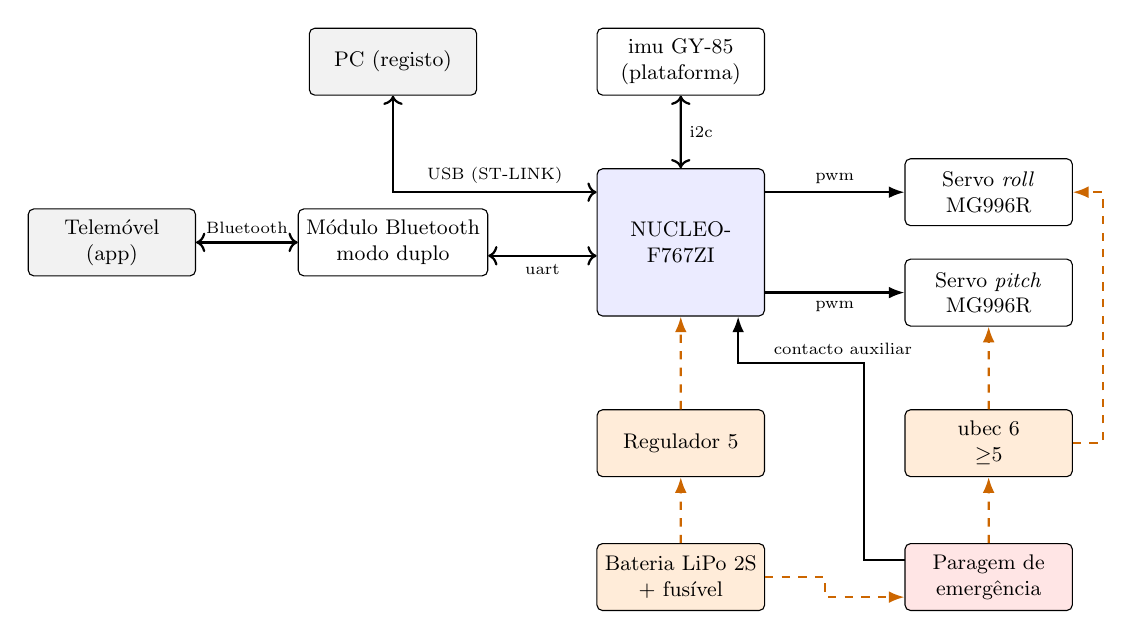
\begin{tikzpicture}[scale=0.85, transform shape,
  bloco/.style={draw, rounded corners=2pt, minimum width=2.5cm, minimum height=1cm, align=center, font=\small},
  pot/.style={bloco, fill=orange!15},
  sinal/.style={-{Latex[length=2mm]}, thick},
  energia/.style={-{Latex[length=2mm]}, thick, orange!80!black, dashed},
  lab/.style={font=\scriptsize}]
\node[bloco, fill=gray!10] (tel) at (-2.3,0) {Telemóvel\\(app)};
\node[bloco] (bt) at (1.9,0) {Módulo Bluetooth\\modo duplo};
\node[bloco, fill=blue!8, minimum height=2.2cm] (mcu) at (6.2,0) {NUCLEO-\\F767ZI};
\node[bloco] (imu) at (6.2,2.7) {\acrshort{imu} GY-85\\(plataforma)};
\node[bloco, fill=gray!10] (pc) at (1.9,2.7) {PC (registo)};
\node[bloco] (s1) at (10.8,0.75) {Servo \textit{roll}\\MG996R};
\node[bloco] (s2) at (10.8,-0.75) {Servo \textit{pitch}\\MG996R};
\node[pot] (reg5) at (6.2,-3.0) {Regulador \SI{5}{\volt}};
\node[pot] (ubec) at (10.8,-3.0) {\acrshort{ubec} \SI{6}{\volt}\\$\geq$\SI{5}{\ampere}};
\node[pot] (bat) at (6.2,-5.0) {Bateria LiPo 2S\\+ fusível};
\node[bloco, fill=red!10] (es) at (10.8,-5.0) {Paragem de\\emergência};

\draw[sinal, <->] (tel) -- node[above, lab]{Bluetooth} (bt);
\draw[sinal, <->] ($(bt.east)+(0,-0.2)$) -- node[below, lab]{\acrshort{uart}} ($(mcu.west)+(0,-0.2)$);
\draw[sinal, <->] (imu) -- node[right, lab]{\acrshort{i2c}} (mcu);
\draw[sinal, <->] (pc.south) |- node[pos=0.75, above, lab]{USB (ST-LINK)} ($(mcu.west)+(0,0.75)$);
\draw[sinal] (mcu.east |- s1) -- node[above, lab]{\acrshort{pwm}} (s1);
\draw[sinal] (mcu.east |- s2) -- node[below, lab]{\acrshort{pwm}} (s2);
\draw[sinal] ($(es.west)+(0,0.25)$) -- ++(-0.6,0) |- node[pos=0.75, above, lab]{contacto auxiliar} (8.3,-1.8) -| ($(mcu.south east)+(-0.4,0)$);
\draw[energia] (bat) -- (reg5);
\draw[energia] (reg5) -- (mcu);
\draw[energia] (bat.east) -- ++(0.9,0) |- ($(es.west)+(0,-0.3)$);
\draw[energia] (es) -- (ubec);
\draw[energia] (ubec) -- (s2);
\draw[energia] (ubec.east) -- ++(0.45,0) |- (s1.east);
\end{tikzpicture}
\caption{Diagrama de blocos do sistema (sinal a cheio, energia a tracejado).}
\label{fig:blocos}
\end{figure}

O sistema tem dois modos de funcionamento previstos. No modo de seguimento, a referência é a inclinação do telemóvel; no modo de nivelamento, a referência é a horizontal e o controlador compensa o movimento da base. Em ambos os casos o controlo é executado localmente, pelo que uma falha da ligação Bluetooth nunca deixa a plataforma sem controlo (RNF6).

\section{Estrutura mecânica}
A estrutura foi modelada em OpenSCAD, de forma paramétrica, e é composta por quatro peças impressas em 3D: a caixa, a tampa com as torres, o quadro do eixo de \textit{roll} e a plataforma do eixo de \textit{pitch} (figuras~\ref{fig:cad-montagem} e~\ref{fig:cad-explodida}). Segue a solução de \textit{gimbal} em série usada nos estabilizadores de câmara: o servo de \textit{roll} está fixo à tampa e roda o quadro, e o servo de \textit{pitch} está fixo ao quadro e roda a plataforma. Os dois eixos cruzam-se no mesmo ponto, \SI{70}{\milli\metre} acima da tampa, pelo que cada servo atua num só ângulo e não há acoplamento mecânico entre eixos.

\begin{figure}[H]
\centering
\begin{subfigure}[b]{0.48\textwidth}
\centering
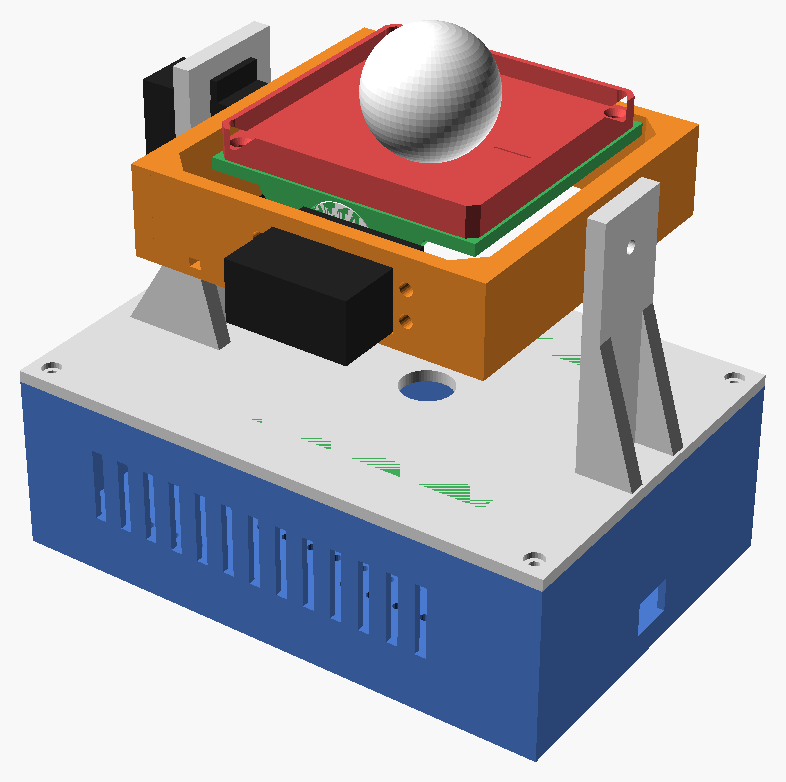
\includegraphics[width=\textwidth]{figuras/montagem.png}
\caption{Posição neutra}
\end{subfigure}\hfill
\begin{subfigure}[b]{0.48\textwidth}
\centering
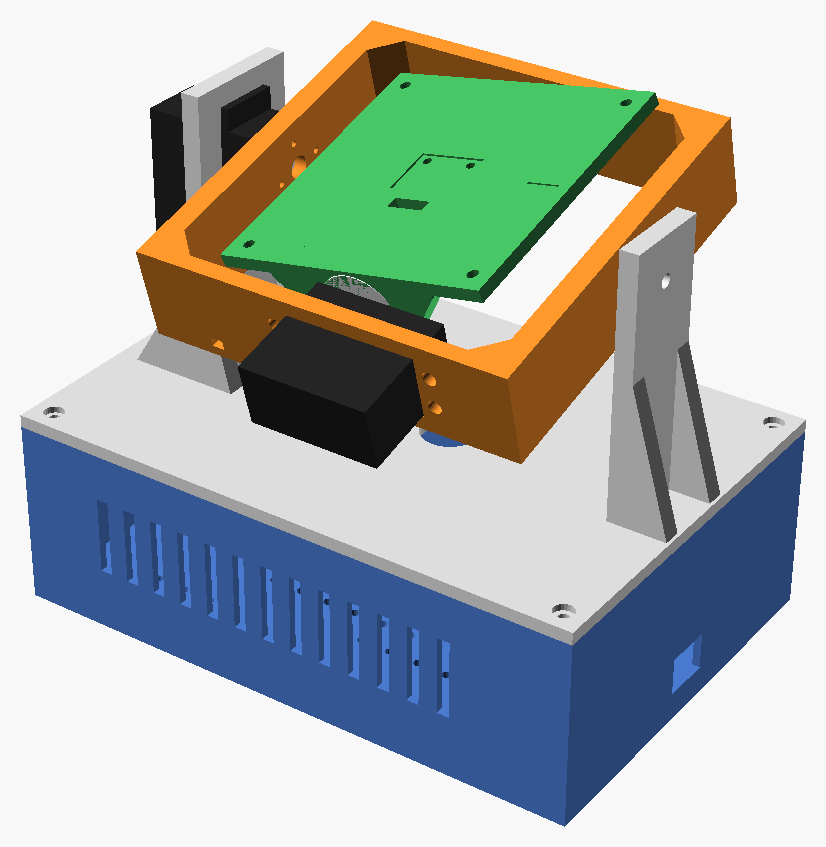
\includegraphics[width=\textwidth]{figuras/montagem_inclinada.png}
\caption{\textit{Roll} de \SI{15}{\degree} e \textit{pitch} de \SI{-12}{\degree}}
\end{subfigure}
\caption{Modelo 3D da plataforma montada (OpenSCAD).}
\label{fig:cad-montagem}
\end{figure}

\begin{figure}[H]
\centering
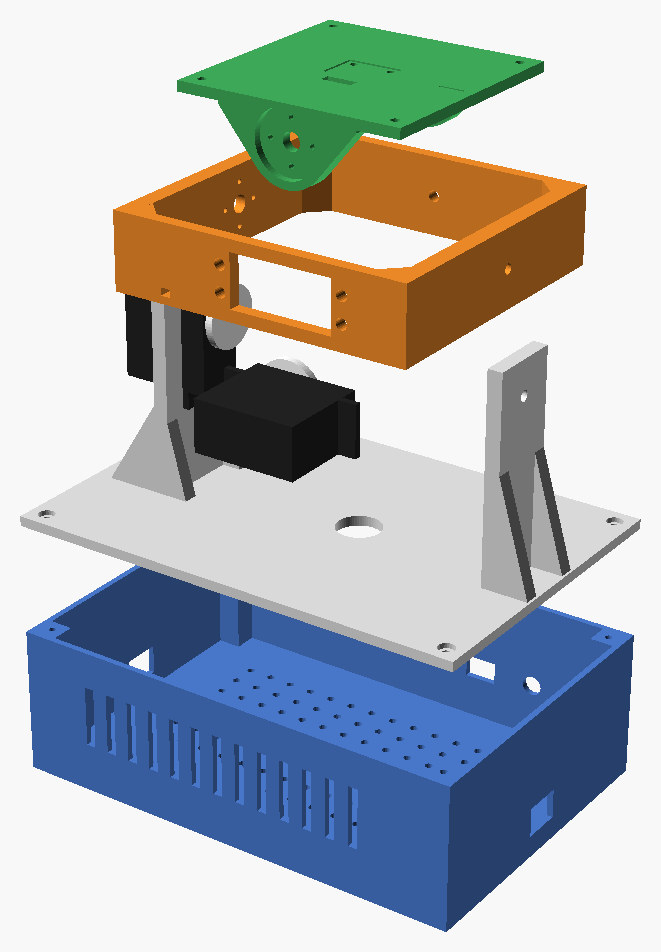
\includegraphics[width=0.55\textwidth]{figuras/explodida.png}
\caption{Vista explodida: caixa (azul), tampa com torres (cinzento), quadro de \textit{roll} (laranja), plataforma de \textit{pitch} (verde) e servos (preto).}
\label{fig:cad-explodida}
\end{figure}

Cada eixo é suportado nos dois lados. Num lado, a peça móvel é aparafusada ao disco (\textit{horn}) do servo, de \SI{25}{\milli\metre} de diâmetro, encaixado num rebaixo de \SI{3}{\milli\metre} e fixo com quatro parafusos M2. No lado oposto, um parafuso M4 funciona como pivô, com uma porca embutida na peça móvel e uma anilha para garantir a folga axial. Assim, o servo não suporta sozinho o peso da peça que roda, o que reduz o esforço no seu veio.

\begin{figure}[H]
\centering
\begin{subfigure}[b]{0.48\textwidth}
\centering
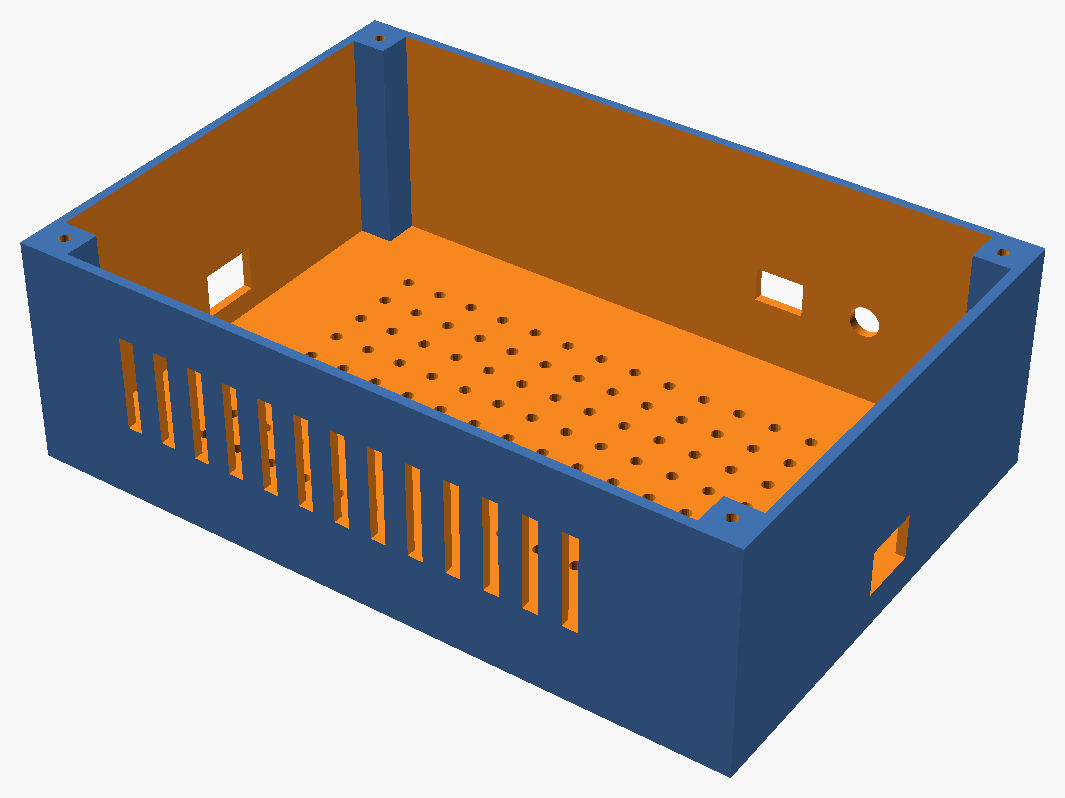
\includegraphics[width=\textwidth]{figuras/peca_caixa.png}
\caption{Caixa}
\end{subfigure}\hfill
\begin{subfigure}[b]{0.48\textwidth}
\centering
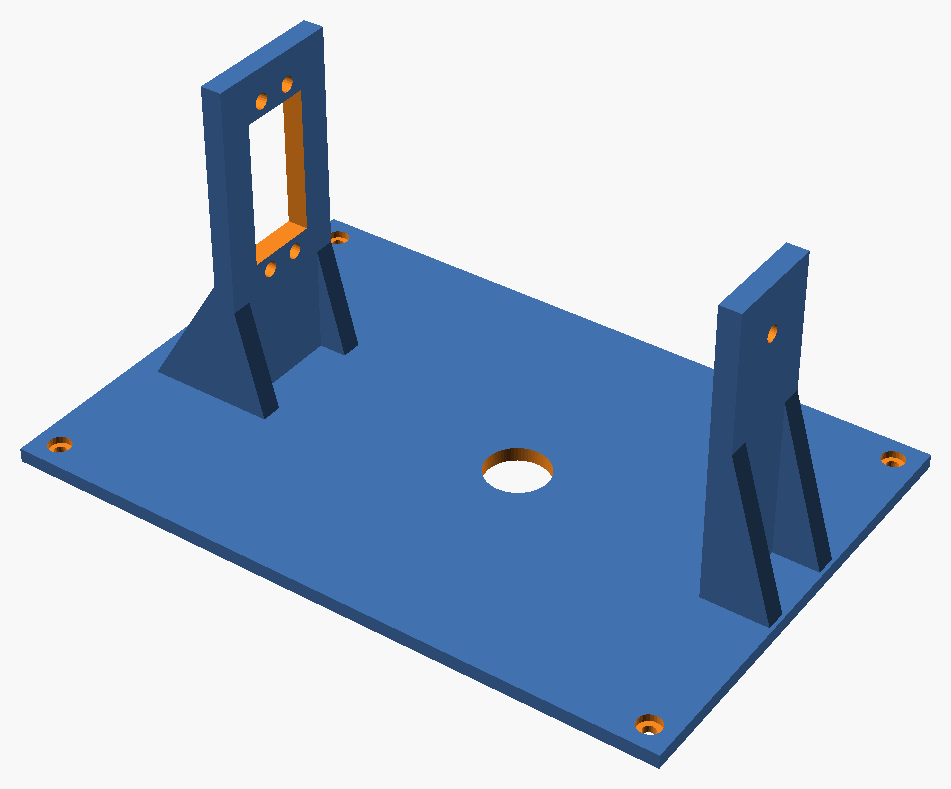
\includegraphics[width=\textwidth]{figuras/peca_tampa.png}
\caption{Tampa com torres}
\end{subfigure}
\\[2mm]
\begin{subfigure}[b]{0.48\textwidth}
\centering
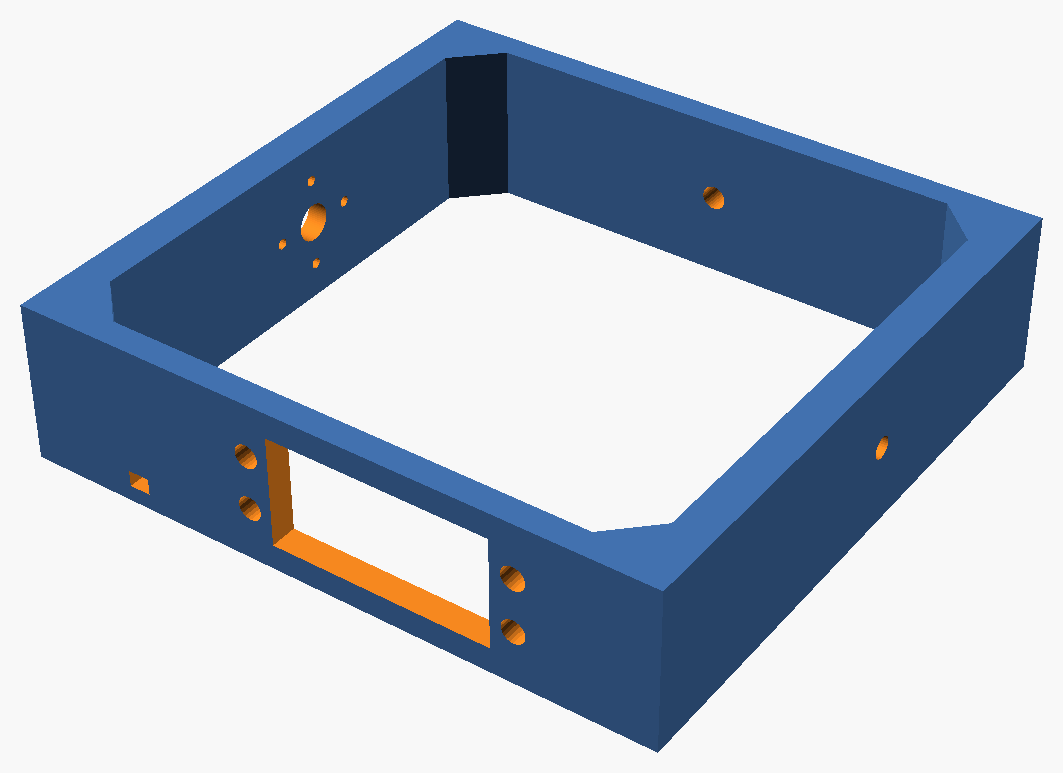
\includegraphics[width=\textwidth]{figuras/peca_quadro.png}
\caption{Quadro do eixo de \textit{roll}}
\end{subfigure}\hfill
\begin{subfigure}[b]{0.48\textwidth}
\centering
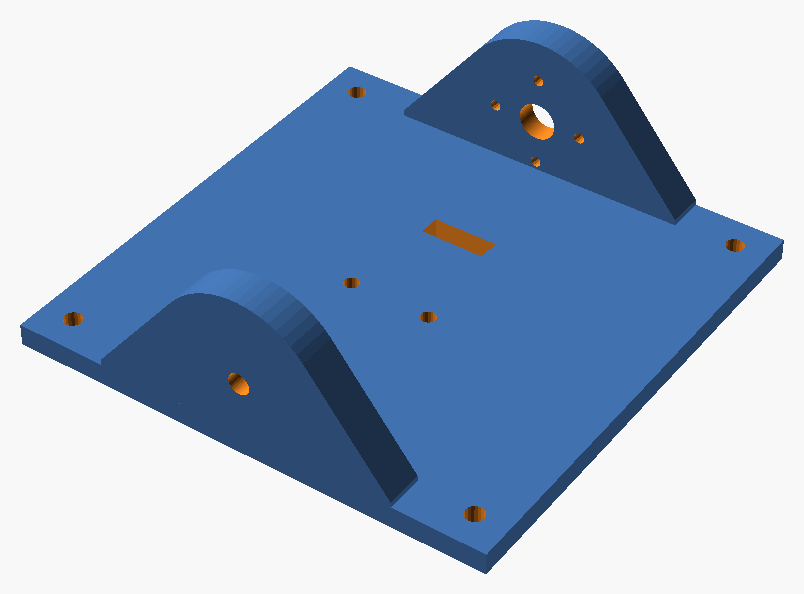
\includegraphics[width=\textwidth]{figuras/peca_plataforma.png}
\caption{Plataforma do eixo de \textit{pitch}}
\end{subfigure}
\caption{Peças impressas em 3D, na orientação de impressão.}
\label{fig:cad-pecas}
\end{figure}

A tabela~\ref{tab:pecas} resume as peças e as suas funções.

\begin{table}[H]
\centering\small
\caption{Peças da estrutura mecânica.}
\begin{tabularx}{\textwidth}{>{\raggedright\arraybackslash}p{2.6cm}>{\raggedright\arraybackslash}p{3.4cm}Y}
\toprule
Peça & Dimensões principais & Função e detalhes\\\midrule
Caixa & $190\times130\times\SI{60}{\milli\metre}$; parede de \SI{2.5}{\milli\metre} & Aloja a NUCLEO, os módulos, os reguladores e a bateria. Fundo com grelha de furos M3 a cada \SI{10}{\milli\metre} para fixar as placas; aberturas para os dois USB da NUCLEO, para a ficha de alimentação e para o interruptor; ranhuras de ventilação\\
Tampa e torres & Tampa de \SI{4}{\milli\metre}; eixos a \SI{70}{\milli\metre} & Torre do servo de \textit{roll} e torre do pivô, com nervuras de reforço; furos de passagem dos cabos; fixação à caixa por quatro parafusos M3\\
Quadro (\textit{roll}) & Moldura de $120\times\SI{115}{\milli\metre}$, paredes de 5 a \SI{7}{\milli\metre} & Ligado ao \textit{horn} do servo de \textit{roll} e ao pivô; transporta o servo de \textit{pitch}; passagem para braçadeira do cabo\\
Plataforma (\textit{pitch}) & $90\times90\times\SI{4}{\milli\metre}$ & Ligada ao \textit{horn} do servo de \textit{pitch} e ao pivô; rebaixo central para a \acrshort{imu}; furos M3 nos cantos para fixar carga; marcação do eixo $x$\\
\bottomrule
\end{tabularx}
\label{tab:pecas}
\end{table}

O modelo usa uma folga de impressão de \SI{0.3}{\milli\metre} e as cotas do MG996R estão parametrizadas, devendo ser confirmadas com paquímetro antes da impressão. O rebaixo da \gls{imu} na plataforma foi desenhado para o módulo GY-521 ($21{,}5\times\SI{16.5}{\milli\metre}$). O GY-85 tem dimensões muito próximas (cerca de $22\times\SI{17}{\milli\metre}$) \cite{gy85}, mas a posição dos furos de fixação tem de ser verificada e ajustada no modelo.

\section{Arquitetura de hardware}

\subsection{Unidade de processamento}
A NUCLEO-F767ZI é alimentada a \SI{5}{\volt} por um regulador dedicado, através da entrada E5V, ou, durante o desenvolvimento, pelo USB do ST-LINK. O ST-LINK disponibiliza também uma porta série virtual, usada para enviar dados de registo para o PC durante os ensaios.

\subsection{Sensor inercial}
O módulo GY-85 é ligado ao barramento \gls{i2c}1 a \SI{400}{\kilo\hertz}. Os três circuitos partilham o barramento, com endereços distintos: ADXL345 em 0x53, ITG-3205 em 0x68 ou 0x69 e HMC5883L em 0x1E \cite{gy85datasheet}. O primeiro teste (IMU-01) é um varrimento do barramento para confirmar os endereços da placa usada.

Propõe-se configurar o acelerómetro em modo de resolução total, na gama de $\pm\SI{2}{g}$, que chega para medir a inclinação, e o giroscópio na gama de $\pm\SI{2000}{\degree\per\second}$, com o filtro passa-baixo digital interno ativo para reduzir o ruído das vibrações dos servos. O magnetómetro não é usado no controlo, mas é configurado para ficar disponível. A leitura é feita por \textit{polling}, sincronizada com o ciclo de \SI{200}{\hertz}.

\subsection{Atuadores}
Os dois servos MG996R são comandados por dois canais do mesmo temporizador, a \SI{50}{\hertz}. Com o relógio do temporizador dividido para \SI{1}{\mega\hertz}, cada unidade corresponde a \SI{1}{\micro\second}, o que dá uma resolução muito superior à banda morta do servo (\SI{5}{\micro\second}) \cite{mg996r}. A largura de impulso é limitada em software a uma janela calibrada, de modo a nunca forçar os batentes mecânicos.

\subsection{Comunicação}
O módulo Bluetooth de modo duplo (HM-12) liga-se à USART6 do microcontrolador \cite{hm12}. Funciona a 9600~bps por omissão. Uma mensagem de referência tem cerca de 25 bytes, o que a esta velocidade ocupa cerca de \SI{26}{\milli\second}; a \SI{20}{\hertz} o canal fica ocupado a cerca de metade. Se o módulo o permitir, a velocidade será aumentada por comando AT para dar margem.

\subsection{Alimentação}
A alimentação é feita por uma bateria LiPo 2S (\SI{7.4}{\volt} nominais, \SI{8.4}{\volt} carregada), protegida por um fusível logo à saída e com um interruptor geral. Os servos são alimentados por um \gls{ubec} de \SI{6}{\volt}, separado da eletrónica para que os picos de corrente não perturbem o microcontrolador nem a \gls{imu}. Como cada MG996R pode consumir \SI{2.5}{\ampere} em bloqueio, o regulador deve fornecer pelo menos \SI{5}{\ampere}; um \gls{ubec} de \SI{3}{\ampere} \cite{hobbywingubec} só serve se o software impedir que os dois servos fiquem bloqueados em simultâneo. Junto aos servos coloca-se um condensador eletrolítico de \SI{1000}{\micro\farad} para absorver os picos. Todas as massas são ligadas num ponto comum.

A tensão da bateria é medida por um divisor resistivo ligado a uma entrada analógica. Com $R_1 = \SI{10}{\kilo\ohm}$ e $R_2 = \SI{4.7}{\kilo\ohm}$, os \SI{8.4}{\volt} da bateria carregada correspondem a \SI{2.69}{\volt} no \gls{adc}, abaixo do limite de \SI{3.3}{\volt}.

A paragem de emergência é um botão com dois contactos normalmente fechados. O primeiro está em série com a alimentação dos servos e corta-a fisicamente quando o botão é atuado. O segundo liga uma entrada digital à massa: em funcionamento normal a entrada lê 0; com o botão atuado o contacto abre, a resistência interna de \textit{pull-up} leva a entrada a 1 e o microcontrolador passa ao estado de falha.

\begin{table}[H]
\centering\small
\caption{Balanço energético estimado.}
\begin{tabularx}{\textwidth}{>{\raggedright\arraybackslash}p{4cm}YYY}
\toprule
Carga & Tensão & Corrente típica & Corrente de pico\\\midrule
2 servos MG996R & \SI{6}{\volt} & \SI{0.5}{\ampere} (total, estimado) & \SI{5}{\ampere} (bloqueio)\\
NUCLEO-F767ZI + \acrshort{imu} + Bluetooth & \SI{5}{\volt} & \SI{0.35}{\ampere} (estimado) & \SI{0.5}{\ampere}\\
\midrule
Potência média & \multicolumn{3}{p{9cm}}{$\approx \SI{3}{\watt} + \SI{1.75}{\watt} \approx \SI{4.8}{\watt}$; cerca de \SI{5.6}{\watt} à saída da bateria, com rendimento de 85\,\% nos reguladores}\\
\bottomrule
\end{tabularx}
\label{tab:energia}
\end{table}

Uma bateria de \SI{2200}{\milli\ampere\hour} armazena cerca de \SI{16}{\watt\hour}. Usando apenas 80\,\% dessa energia, a autonomia estimada é de $16 \times 0{,}8 / 5{,}6 \approx \SI{2.3}{\hour}$, bem acima dos \SI{30}{\minute} do requisito RNF7. As correntes típicas são estimativas e serão medidas no ensaio T-ALIM.

\section{Esquema elétrico}
O esquema elétrico está dividido em duas partes: as ligações de sinal entre a NUCLEO e os módulos (figura~\ref{fig:esq-sinal}) e o circuito de alimentação (figura~\ref{fig:esq-alim}). Nas figuras, os nomes \texttt{+5V}, \texttt{+6V\_SERVO}, \texttt{VBAT\_ADC} e GND indicam ligações à mesma rede. A tabela~\ref{tab:pinos} resume os pinos usados.

\begin{figure}[H]
\centering
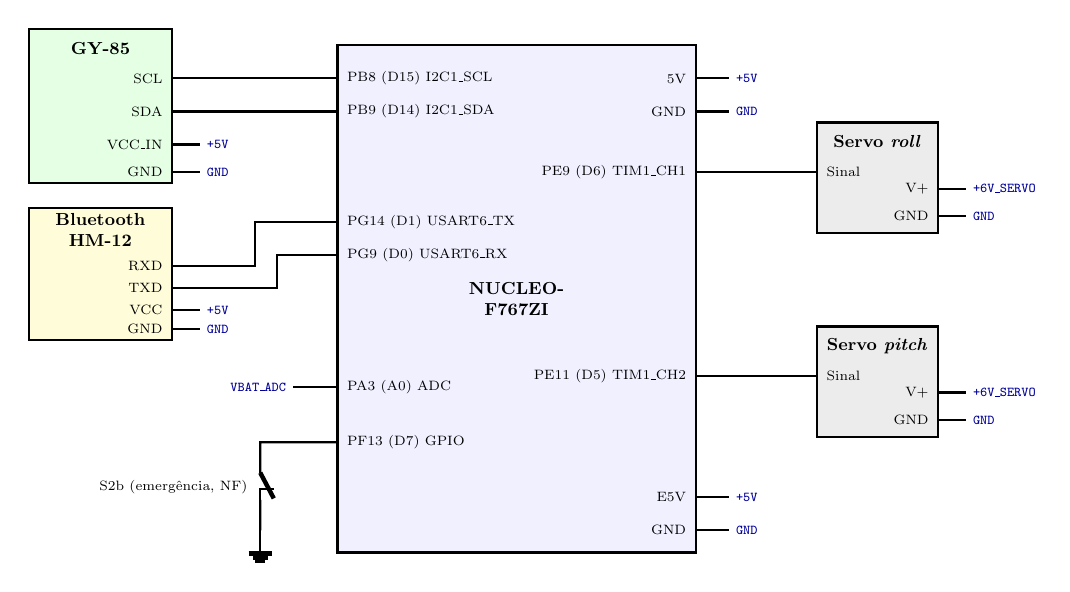
\begin{tikzpicture}[scale=0.70, transform shape,
  pin/.style={font=\scriptsize},
  tit/.style={font=\small\bfseries, align=center},
  net/.style={font=\scriptsize\ttfamily, text=blue!60!black},
  fio/.style={thick}]
% ---------------- NUCLEO ----------------
\draw[thick, fill=blue!6] (6,-4.6) rectangle (12.5,4.6);
\node[tit] at (9.25,0) {NUCLEO-\\F767ZI};
\foreach \y/\t in {4.0/{PB8 (D15) I2C1\_SCL}, 3.4/{PB9 (D14) I2C1\_SDA}, 1.4/{PG14 (D1) USART6\_TX}, 0.8/{PG9 (D0) USART6\_RX}, -1.6/{PA3 (A0) ADC}, -2.6/{PF13 (D7) GPIO}}
  {\node[pin, anchor=west] at (6.05,\y) {\t};}
\foreach \y/\t in {4.0/{5V}, 3.4/{GND}, 2.3/{PE9 (D6) TIM1\_CH1}, -1.4/{PE11 (D5) TIM1\_CH2}, -3.6/{E5V}, -4.2/{GND}}
  {\node[pin, anchor=east] at (12.45,\y) {\t};}
% ---------------- GY-85 ----------------
\draw[thick, fill=green!10] (0.4,2.1) rectangle (3.0,4.9);
\node[tit] at (1.7,4.55) {GY-85};
\foreach \y/\t in {4.0/SCL, 3.4/SDA, 2.8/VCC\_IN, 2.3/GND}{\node[pin, anchor=east] at (2.95,\y) {\t};}
\draw[fio] (3,4.0) -- (6,4.0);
\draw[fio] (3,3.4) -- (6,3.4);
\draw[fio] (3,2.8) -- (3.5,2.8) node[net, right]{+5V};
\draw[fio] (3,2.3) -- (3.5,2.3) node[net, right]{GND};
% ---------------- HM-12 ----------------
\draw[thick, fill=yellow!15] (0.4,-0.75) rectangle (3.0,1.65);
\node[tit] at (1.7,1.25) {Bluetooth\\HM-12};
\foreach \y/\t in {0.6/RXD, 0.2/TXD, -0.2/VCC, -0.55/GND}{\node[pin, anchor=east] at (2.95,\y) {\t};}
\draw[fio] (3,0.6) -- (4.5,0.6) |- (6,1.4);
\draw[fio] (3,0.2) -- (4.9,0.2) |- (6,0.8);
\draw[fio] (3,-0.2) -- (3.5,-0.2) node[net, right]{+5V};
\draw[fio] (3,-0.55) -- (3.5,-0.55) node[net, right]{GND};
% ---------------- ADC e emergência ----------------
\draw[fio] (6,-1.6) -- (5.2,-1.6) node[net, left]{VBAT\_ADC};
\draw[fio] (6,-2.6) -- (4.6,-2.6) to[ncs, l_={\scriptsize S2b (emergência, NF)}] (4.6,-4.2) node[ground]{};
% ---------------- alimentação da NUCLEO ----------------
\draw[fio] (12.5,4.0) -- (13.1,4.0) node[net, right]{+5V};
\draw[fio] (12.5,3.4) -- (13.1,3.4) node[net, right]{GND};
\draw[fio] (12.5,-3.6) -- (13.1,-3.6) node[net, right]{+5V};
\draw[fio] (12.5,-4.2) -- (13.1,-4.2) node[net, right]{GND};
% ---------------- Servos ----------------
\foreach \ys/\nome in {2.3/{Servo \textit{roll}}, -1.4/{Servo \textit{pitch}}}{
  \draw[thick, fill=gray!15] (14.7,\ys-1.1) rectangle (16.9,\ys+0.9);
  \node[tit] at (15.8,\ys+0.55) {\nome};
  \node[pin, anchor=west] at (14.75,\ys) {Sinal};
  \node[pin, anchor=east] at (16.85,\ys-0.3) {V+};
  \node[pin, anchor=east] at (16.85,\ys-0.8) {GND};
  \draw[fio] (16.9,\ys-0.3) -- (17.4,\ys-0.3) node[net, right]{+6V\_SERVO};
  \draw[fio] (16.9,\ys-0.8) -- (17.4,\ys-0.8) node[net, right]{GND};
  \draw[fio] (12.5,\ys) -- (14.7,\ys);
}
\end{tikzpicture}
\caption{Esquema elétrico: ligações de sinal entre a NUCLEO-F767ZI e os módulos.}
\label{fig:esq-sinal}
\end{figure}

\begin{figure}[H]
\centering
\begin{circuitikz}[scale=0.85, transform shape, font=\small]
% bateria, fusível e interruptor
\draw (0,0) to[battery1, l={Bateria LiPo 2S}, a={\SI{7.4}{\volt}}, invert] (0,3)
      to[fuse, l={F1}] (2.6,3)
      to[spst, l={SW1}] (5,3) node[circ]{};
\node[above, font=\scriptsize\ttfamily, text=blue!60!black] at (5,3.05) {VBAT};
% divisor de tensão
\draw (5,3) to[R, l_={$R_1$ \SI{10}{\kilo\ohm}}] (5,1.5) node[circ]{}
      to[R, l_={$R_2$ \SI{4.7}{\kilo\ohm}}] (5,0);
\draw (5,1.5) -- (5.9,1.5) node[right, font=\scriptsize\ttfamily, text=blue!60!black]{VBAT\_ADC};
% regulador 5 V
\draw (5,3) -- (7.2,3);
\draw[thick, fill=orange!15] (7.2,2.4) rectangle (9.4,3.6);
\node[align=center, font=\scriptsize] at (8.3,3) {Regulador\\\textit{buck} \SI{5}{\volt}};
\draw (8.3,2.4) -- (8.3,0);
\draw (9.4,3) -- (10.2,3) node[right, font=\scriptsize\ttfamily, text=blue!60!black]{+5V};
% ramo dos servos com emergência
\draw (5,3) -- (5,5) to[ncs] (7.2,5);
\node[font=\scriptsize, align=center] at (6.1,5.75) {S2a: emergência (NF)};
\draw (7.2,5) -- (8.4,5);
\draw[thick, fill=orange!15] (8.4,4.4) rectangle (10.6,5.6);
\node[align=center, font=\scriptsize] at (9.5,5) {\acrshort{ubec}\\\SI{6}{\volt}, $\geq$\SI{5}{\ampere}};
\draw (9.5,4.4) -- (9.5,4.1) -- (11.3,4.1) -- (11.3,0);
\draw (10.6,5) -- (12.4,5) to[C, l={$C_1$ \SI{1000}{\micro\farad}}] (12.4,0);
\draw (12.4,5) -- (13.2,5) node[right, font=\scriptsize\ttfamily, text=blue!60!black]{+6V\_SERVO};
% massa
\draw (0,0) -- (12.4,0);
\draw (6.2,0) node[ground]{};
\end{circuitikz}
\caption{Esquema elétrico: circuito de alimentação. S2a e S2b são os dois contactos normalmente fechados do mesmo botão de emergência.}
\label{fig:esq-alim}
\end{figure}

\begin{table}[H]
\centering\small
\caption{Atribuição de pinos (NUCLEO-F767ZI).}
\begin{tabularx}{\textwidth}{>{\raggedright\arraybackslash}p{3.4cm}>{\raggedright\arraybackslash}p{2.6cm}>{\raggedright\arraybackslash}p{2.8cm}Y}
\toprule
Sinal & Pino & Periférico & Ligação\\\midrule
\acrshort{i2c} SCL & PB8 (D15) & I2C1 & GY-85 SCL\\
\acrshort{i2c} SDA & PB9 (D14) & I2C1 & GY-85 SDA\\
\acrshort{pwm} servo \textit{roll} & PE9 (D6) & TIM1\_CH1 & Sinal do servo 1\\
\acrshort{pwm} servo \textit{pitch} & PE11 (D5) & TIM1\_CH2 & Sinal do servo 2\\
\acrshort{uart} TX & PG14 (D1) & USART6 & RXD do módulo Bluetooth\\
\acrshort{uart} RX & PG9 (D0) & USART6 & TXD do módulo Bluetooth\\
Tensão da bateria & PA3 (A0) & \acrshort{adc} & Divisor resistivo ($R_1$, $R_2$)\\
Paragem de emergência & PF13 (D7) & GPIO com \textit{pull-up} & Contacto auxiliar S2b\\
Alimentação & E5V & -- & Saída do regulador de \SI{5}{\volt}\\
\acrshort{led} de estado & PB0, PB7, PB14 & GPIO & \acrshort{led} da placa (LD1--LD3)\\
\bottomrule
\end{tabularx}
\label{tab:pinos}
\end{table}

Os pinos foram escolhidos nos conectores compatíveis com Arduino da placa, o que facilita a cablagem com fios Dupont, e devem ser confirmados com o manual da NUCLEO antes da montagem. Para alimentar a placa pela entrada E5V é necessário mudar o \textit{jumper} de seleção de alimentação. O GY-85 e o módulo Bluetooth são alimentados a partir do pino de \SI{5}{\volt} da NUCLEO; o GY-85 tem regulador próprio e o módulo Bluetooth deve ter a gama de tensão confirmada na respetiva ficha técnica.

\section{Arquitetura de software}

\subsection{Organização em camadas}
O software está organizado em três camadas (figura~\ref{fig:camadas}). A camada inferior é a biblioteca \gls{hal} do fabricante, que dá acesso aos periféricos. Por cima dela ficam os controladores de dispositivo (\textit{drivers}), um por componente, que escondem os detalhes de cada circuito. A camada de serviços contém a fusão sensorial, o controlo, o protocolo de comunicação, a supervisão e o registo. A aplicação, no topo, implementa a máquina de estados que coordena tudo.

\begin{figure}[H]
\centering
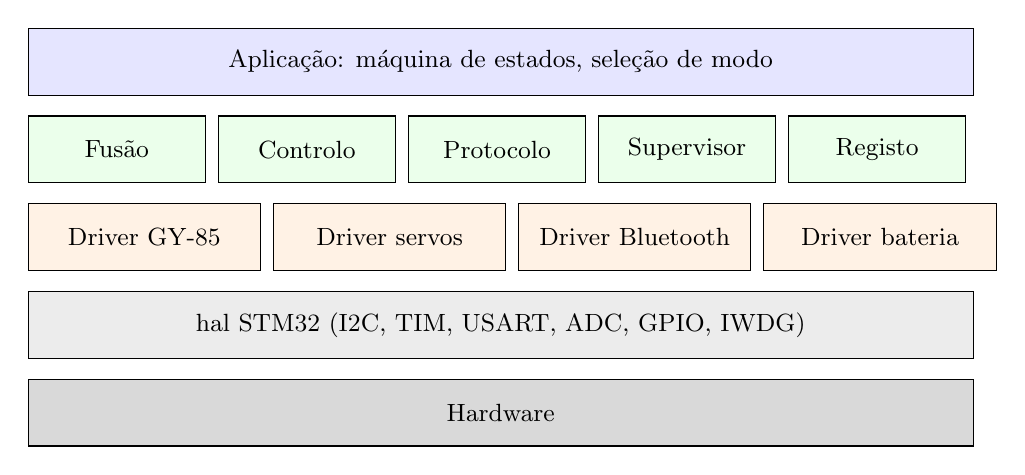
\begin{tikzpicture}[
  cam/.style={draw, minimum height=0.85cm, align=center, font=\small},
  node distance=0.15cm]
\node[cam, minimum width=12cm, fill=blue!10] (app) {Aplicação: máquina de estados, seleção de modo};
\node[cam, minimum width=2.25cm, below=0.25cm of app.south west, anchor=north west, fill=green!8] (fus) {Fusão};
\node[cam, minimum width=2.25cm, right=of fus, fill=green!8] (ctl) {Controlo};
\node[cam, minimum width=2.25cm, right=of ctl, fill=green!8] (prot) {Protocolo};
\node[cam, minimum width=2.25cm, right=of prot, fill=green!8] (sup) {Supervisor};
\node[cam, minimum width=2.25cm, right=of sup, fill=green!8] (log) {Registo};
\node[cam, minimum width=2.95cm, below=0.25cm of fus.south west, anchor=north west, fill=orange!10] (dimu) {Driver GY-85};
\node[cam, minimum width=2.95cm, right=of dimu, fill=orange!10] (dsrv) {Driver servos};
\node[cam, minimum width=2.95cm, right=of dsrv, fill=orange!10] (dbt) {Driver Bluetooth};
\node[cam, minimum width=2.95cm, right=of dbt, fill=orange!10] (dadc) {Driver bateria};
\node[cam, minimum width=12cm, below=0.25cm of dimu.south west, anchor=north west, fill=gray!15] (hal) {\acrshort{hal} STM32 (I2C, TIM, USART, ADC, GPIO, IWDG)};
\node[cam, minimum width=12cm, below=0.25cm of hal.south west, anchor=north west, fill=gray!30] (hw) {Hardware};
\end{tikzpicture}
\caption{Camadas do software.}
\label{fig:camadas}
\end{figure}

Esta organização permite testar cada módulo isoladamente (capítulo~\ref{ch:testes}) e trocar um componente, por exemplo a \gls{imu}, alterando apenas o respetivo \textit{driver}. Foi o que aconteceu na passagem da MPU6050 para o GY-85, que só afeta o \textit{driver} do sensor.

\subsection{Execução e temporização}
O software não usa sistema operativo. A temporização é garantida por um temporizador que gera uma interrupção a \SI{200}{\hertz} (\SI{5}{\milli\second}). Em cada interrupção lê-se a \gls{imu}, atualiza-se a estimativa de atitude e corre-se o supervisor. O controlador corre a \SI{50}{\hertz}, sincronizado com o período do sinal \gls{pwm}, porque não adianta calcular comandos mais depressa do que o servo os consegue receber. Esta separação segue a prática dos controladores de voo, em que a estimação e o controlo correm a frequências diferentes \cite{px4ctrl,ardupilotatt}.

A receção da porta série é feita por interrupção para um \textit{buffer} circular. A interpretação das mensagens, o envio de telemetria e o registo correm no ciclo principal, fora das interrupções, para não atrasar o controlo. Um \textit{watchdog} independente (IWDG) é renovado em cada ciclo de controlo: se o programa bloquear, o microcontrolador reinicia e arranca no estado seguro.

\begin{table}[H]
\centering\small
\caption{Tarefas e frequências de execução.}
\begin{tabularx}{\textwidth}{>{\raggedright\arraybackslash}p{4cm}p{2.2cm}Y}
\toprule
Tarefa & Frequência & Contexto\\\midrule
Leitura da \acrshort{imu} e fusão & \SI{200}{\hertz} & Interrupção do temporizador\\
Supervisor (limites, \textit{timeouts}) & \SI{200}{\hertz} & Interrupção do temporizador\\
Controlo e atualização dos servos & \SI{50}{\hertz} & Interrupção do temporizador (1 em cada 4)\\
Receção Bluetooth & Por byte & Interrupção da USART\\
Interpretação de mensagens & Contínua & Ciclo principal\\
Telemetria para o telemóvel & \SI{5}{\hertz} & Ciclo principal\\
Registo para o PC & \SI{50}{\hertz} & Ciclo principal\\
Leitura da bateria & \SI{1}{\hertz} & Ciclo principal\\
\bottomrule
\end{tabularx}
\label{tab:tarefas}
\end{table}

\subsection{Malha de controlo}
A figura~\ref{fig:malha} mostra a malha de controlo de um eixo. A referência $r$ é a inclinação do telemóvel (modo de seguimento) ou zero (modo de nivelamento). Antes de chegar ao controlador, a referência passa por um limitador de amplitude e de velocidade. O controlador \gls{pid} calcula a correção, à qual se pode somar uma compensação antecipativa da inclinação da base, medida por uma segunda \gls{imu}, se for instalada. O comando final é saturado e convertido em largura de impulso através da calibração do servo.

\begin{figure}[H]
\centering
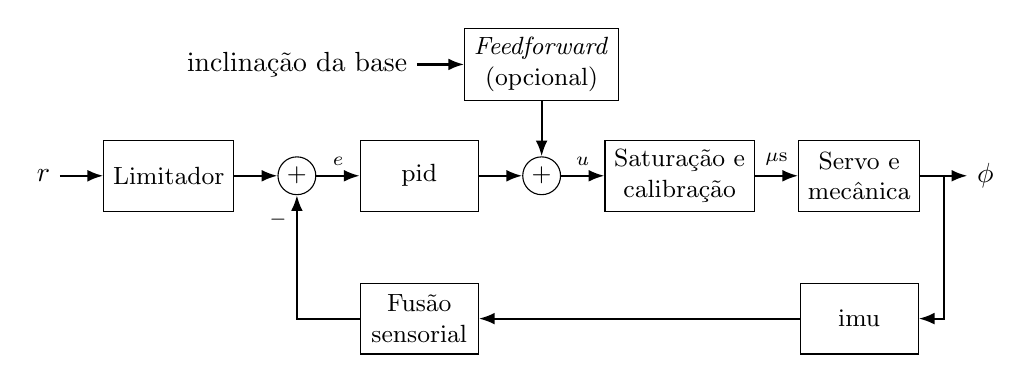
\begin{tikzpicture}[
  bl/.style={draw, minimum height=0.9cm, minimum width=1.5cm, align=center, font=\small},
  sum/.style={draw, circle, inner sep=1.5pt, font=\small},
  sig/.style={-{Latex[length=2mm]}, thick},
  node distance=0.55cm]
\node (r) {$r$};
\node[bl, right=of r] (lim) {Limitador};
\node[sum, right=of lim] (s1) {$+$};
\node[bl, right=of s1] (pid) {\acrshort{pid}};
\node[sum, right=of pid] (s2) {$+$};
\node[bl, right=of s2] (sat) {Saturação e\\calibração};
\node[bl, right=of sat] (servo) {Servo e\\mecânica};
\node[right=0.6cm of servo] (y) {$\phi$};
\node[bl, below=0.9cm of pid] (fus) {Fusão\\sensorial};
\node[bl, below=0.9cm of servo] (imu) {\acrshort{imu}};
\node[bl, above=0.7cm of s2] (ff) {\textit{Feedforward}\\(opcional)};
\node[left=0.6cm of ff] (base) {inclinação da base};
\draw[sig] (r) -- (lim);
\draw[sig] (lim) -- (s1);
\draw[sig] (s1) -- node[above, font=\scriptsize]{$e$} (pid);
\draw[sig] (pid) -- (s2);
\draw[sig] (s2) -- node[above, font=\scriptsize]{$u$} (sat);
\draw[sig] (sat) -- node[above, font=\scriptsize]{$\mu$s} (servo);
\draw[sig] (servo) -- (y);
\draw[sig] ($(servo.east)+(0.3,0)$) |- (imu);
\draw[sig] (imu) -- (fus);
\draw[sig] (fus) -| node[pos=0.9, left, font=\scriptsize]{$-$} (s1);
\draw[sig] (base) -- (ff);
\draw[sig] (ff) -- (s2);
\end{tikzpicture}
\caption{Malha de controlo de um eixo.}
\label{fig:malha}
\end{figure}

O termo integral é limitado e congelado sempre que o comando satura, para evitar \textit{windup}. O termo derivativo é calculado sobre a medida, e não sobre o erro, para evitar picos quando a referência muda bruscamente, e é filtrado por um passa-baixo. Ao mudar de modo, o integrador é inicializado com o comando atual, para que a transição não provoque saltos (RF5).

Com o \textit{gimbal} em série, o ângulo de cada eixo é igual ao ângulo do veio do respetivo servo, a menos de um desvio de montagem. Usa-se, por isso, uma relação linear por eixo, $t = t_0 + k\,u$, em que $t_0$ é a largura de impulso que deixa a plataforma horizontal e $k$ o ganho em \si[per-mode=symbol]{\micro\second\per\degree}, ambos obtidos no ensaio de calibração T-SRV.

\subsection{Máquina de estados}
A figura~\ref{fig:estados} mostra a máquina de estados da aplicação. O sistema arranca sempre desarmado, com os servos na posição neutra, e só passa a controlar a plataforma depois de calibrado e de receber uma ordem explícita para armar, à semelhança do que acontece nos drones.

\begin{figure}[H]
\centering
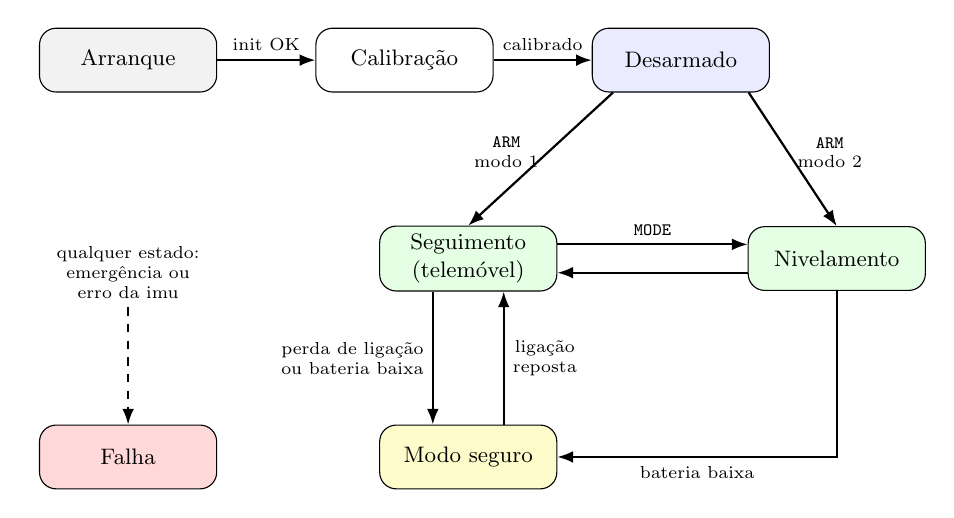
\begin{tikzpicture}[scale=0.9, transform shape,
  est/.style={draw, rounded corners=6pt, minimum width=2.5cm, minimum height=0.9cm, align=center, font=\small},
  tr/.style={-{Latex[length=2mm]}, thick},
  lab/.style={font=\scriptsize, align=center}]
\node[est, fill=gray!10] (arr) at (0,0) {Arranque};
\node[est] (cal) at (3.9,0) {Calibração};
\node[est, fill=blue!8] (des) at (7.8,0) {Desarmado};
\node[est, fill=green!10] (seg) at (4.8,-2.8) {Seguimento\\(telemóvel)};
\node[est, fill=green!10] (niv) at (10.0,-2.8) {Nivelamento};
\node[est, fill=yellow!20] (seguro) at (4.8,-5.6) {Modo seguro};
\node[est, fill=red!15] (falha) at (0,-5.6) {Falha};
\node[lab, text width=2.6cm] (qq) at (0,-3.0) {qualquer estado:\\emergência ou\\erro da \acrshort{imu}};

\draw[tr] (arr) -- node[above, lab]{init OK} (cal);
\draw[tr] (cal) -- node[above, lab]{calibrado} (des);
\draw[tr] (des.south west) ++(0.3,0) -- node[left, lab, pos=0.45]{\texttt{ARM}\\modo 1} (seg.north);
\draw[tr] (des.south east) ++(-0.3,0) -- node[right, lab, pos=0.45]{\texttt{ARM}\\modo 2} (niv.north);
\draw[tr] ([yshift=2mm]seg.east) -- node[above, lab]{\texttt{MODE}} ([yshift=2mm]niv.west);
\draw[tr] ([yshift=-2mm]niv.west) -- ([yshift=-2mm]seg.east);
\draw[tr] ([xshift=-5mm]seg.south) -- node[left, lab]{perda de ligação\\ou bateria baixa} ([xshift=-5mm]seguro.north);
\draw[tr] ([xshift=5mm]seguro.north) -- node[right, lab]{ligação\\reposta} ([xshift=5mm]seg.south);
\draw[tr] (niv.south) |- node[pos=0.75, below, lab]{bateria baixa} (seguro.east);
\draw[tr, dashed] (qq) -- (falha);
\end{tikzpicture}
\caption{Máquina de estados da aplicação. Em qualquer estado armado, \texttt{DISARM} leva ao estado Desarmado.}
\label{fig:estados}
\end{figure}

\begin{table}[H]
\centering\small
\caption{Estados da aplicação.}
\begin{tabularx}{\textwidth}{>{\raggedright\arraybackslash}p{2.6cm}Yp{3.2cm}}
\toprule
Estado & Comportamento & \acrshort{led}\\\midrule
Arranque & Inicializa periféricos e verifica a comunicação com os três sensores do GY-85 & Todos acesos\\
Calibração & Com a plataforma parada, mede o desvio do giroscópio durante alguns segundos & Azul intermitente\\
Desarmado & Servos na posição neutra; aguarda ordem para armar & Azul fixo\\
Seguimento & Segue a inclinação do telemóvel, com limites de amplitude e velocidade & Verde fixo\\
Nivelamento & Mantém a plataforma horizontal & Verde intermitente\\
Modo seguro & Entra por perda de ligação ou bateria baixa; leva a referência a zero com rampa suave e aguarda nova ligação ou ordem para desarmar & Vermelho intermitente\\
Falha & Entra por emergência ou erro da \acrshort{imu}; servos sem comando (ou sem alimentação, se for emergência); exige reinício & Vermelho fixo\\
\bottomrule
\end{tabularx}
\label{tab:estados}
\end{table}

\subsection{Protocolo de comunicação}
As mensagens são linhas de texto ASCII, com um formato inspirado no NMEA: começam por \texttt{\$}, têm campos separados por vírgulas e terminam com \texttt{*}, um \textit{checksum} de dois dígitos hexadecimais (XOR dos caracteres entre \texttt{\$} e \texttt{*}) e fim de linha. O texto facilita a depuração com uma aplicação genérica de terminal Bluetooth e o \textit{checksum} permite rejeitar mensagens corrompidas.

\begin{table}[H]
\centering\small
\caption{Mensagens do protocolo.}
\begin{tabularx}{\textwidth}{>{\raggedright\arraybackslash}p{1.7cm}p{1.4cm}>{\raggedright\arraybackslash}p{5.2cm}Y}
\toprule
Mensagem & Sentido & Exemplo & Significado\\\midrule
REF & T $\rightarrow$ P & \texttt{\$REF,-12.5,4.3,57*63} & Referência de \textit{roll} e \textit{pitch} em graus e número de sequência\\
MODE & T $\rightarrow$ P & \texttt{\$MODE,1*1E} & Seleção de modo (1 seguimento, 2 nivelamento)\\
ARM & T $\rightarrow$ P & \texttt{\$ARM*5E} / \texttt{\$DISARM*00} & Armar ou desarmar\\
CAL & T $\rightarrow$ P & \texttt{\$CAL*4E} & Pedir nova calibração (só desarmado)\\
TEL & P $\rightarrow$ T & \texttt{\$TEL,1.2,-0.4,1,3*75} & Atitude medida, modo e estado\\
\bottomrule
\end{tabularx}
\label{tab:protocolo}
\end{table}

Uma referência é aceite apenas se o \textit{checksum} estiver correto, se os ângulos estiverem dentro da gama de movimento e se o número de sequência for mais recente do que o anterior. Se não chegar nenhuma referência válida durante \SI{300}{\milli\second}, o supervisor passa ao modo seguro, o que cumpre o requisito RNF5 com margem.

\subsection{Aplicação do telemóvel}
Numa primeira fase, os ensaios de comunicação são feitos com uma aplicação genérica de terminal Bluetooth, enviando mensagens escritas à mão. A aplicação final lê a orientação do telemóvel através dos sensores do sistema operativo \cite{android}, calcula \textit{roll} e \textit{pitch} em relação a uma posição neutra definida pelo utilizador e envia as mensagens \texttt{REF} a \SI{20}{\hertz}.

\acompletar{ferramenta usada para a aplicação (por exemplo, Android Studio ou MIT App Inventor) e capturas de ecrã}

\section{Módulos do sistema}
A tabela~\ref{tab:modulos} resume os módulos de software, as respetivas responsabilidades e interfaces.

\begin{table}[H]
\centering\small
\caption{Módulos do sistema e respetivas interfaces.}
\begin{tabularx}{\textwidth}{>{\raggedright\arraybackslash}p{2.3cm}YYY}
\toprule
Módulo & Responsabilidade & Entradas & Saídas\\\midrule
Driver GY-85 & Configurar o ADXL345, o ITG-3205 e o HMC5883L e ler as medidas & Barramento \acrshort{i2c} & $a_{x,y,z}$ em $g$, $\omega_{x,y,z}$ em \si{\degree\per\second}, campo magnético\\
Fusão & Estimar \textit{roll} e \textit{pitch}; calibrar o desvio do giroscópio & Dados da \acrshort{imu}, $\Delta t$ & $\phi$, $\theta$ em graus\\
Controlo & Calcular o comando de cada eixo & Referência, atitude, ganhos & Ângulo de comando por eixo\\
Driver servos & Converter ângulo em largura de impulso e gerar o \acrshort{pwm} & Ângulo de comando, calibração & Sinais \acrshort{pwm}\\
Driver Bluetooth & Receber e enviar bytes pela \acrshort{uart} & \acrshort{uart} & \textit{Buffer} de receção\\
Protocolo & Interpretar e validar mensagens; gerar telemetria & \textit{Buffer} de receção & Referências e comandos validados\\
Supervisor & Verificar \textit{timeouts}, limites, bateria e emergência & Estado de todos os módulos & Eventos para a máquina de estados\\
Aplicação & Gerir estados e modos & Eventos, comandos & Modo ativo, \acrshort{led}\\
Registo & Enviar dados para o PC durante os ensaios & Variáveis internas & Linhas CSV pela porta série do ST-LINK\\
\bottomrule
\end{tabularx}
\label{tab:modulos}
\end{table}

\chapter{Procedimentos e Vetores de Teste}
\label{ch:testes}

Cada módulo é testado isoladamente antes da integração, seguindo a organização do capítulo~\ref{ch:arquitetura}. Para cada módulo define-se o objetivo, o procedimento e um conjunto de vetores de teste, ou seja, entradas concretas com o resultado esperado e o critério de aceitação. Os identificadores dos testes ligam-se aos requisitos das tabelas~\ref{tab:rf} e~\ref{tab:rnf}. As tolerâncias são valores iniciais e podem ser ajustadas depois dos primeiros ensaios.

\section{Metodologia e equipamento}
Os testes usam o seguinte equipamento: um inclinómetro digital (ou um telemóvel com aplicação de nível, previamente comparado com uma superfície de referência) para medir a inclinação real; uma superfície inclinável com ângulos fixos de referência; um multímetro; um osciloscópio ou analisador lógico para os sinais \gls{pwm}, \gls{i2c} e \gls{uart}; e um PC que recebe os dados de registo pela porta série do ST-LINK.

Cada ensaio de medida é repetido pelo menos cinco vezes e são registados a média e o desvio-padrão. Os dados de registo são guardados em ficheiros CSV, para que os gráficos e as métricas possam ser recalculados.

\section{Sensor inercial (T-IMU)}
\textbf{Objetivo:} verificar a comunicação com os três sensores do GY-85, a escala das medidas e o ruído em repouso (RF1, RF6).

\textbf{Procedimento:} fazer um varrimento do barramento \gls{i2c} e ler os registos de identificação de cada sensor. Com o módulo fixo numa superfície plana, registar 10~s de dados a \SI{200}{\hertz}. Repetir com o sensor orientado segundo cada um dos seis sentidos dos eixos, para verificar que o acelerómetro mede $\pm1\,g$ no eixo vertical.

\begin{table}[H]
\centering\small
\caption{Vetores de teste do sensor inercial.}
\begin{tabularx}{\textwidth}{p{1.6cm}YYY}
\toprule
ID & Entrada & Resultado esperado & Critério de aceitação\\\midrule
IMU-01 & Varrimento do barramento \acrshort{i2c} & Respostas em 0x53, 0x68 (ou 0x69) e 0x1E & Três dispositivos encontrados; endereços registados\\
IMU-02 & Leitura do registo DEVID do ADXL345 & 0xE5 & Valor igual\\
IMU-03 & Leitura do registo WHO\_AM\_I do ITG-3205 & Igual ao endereço do giroscópio & Valor igual\\
IMU-04 & Leitura dos registos de identificação do HMC5883L & \texttt{H}, \texttt{4}, \texttt{3} & Valores iguais (caso contrário, verificar se é QMC5883L)\\
IMU-05 & Sensor horizontal, eixo $z$ para cima & $a_z = +1\,g$; $a_x$, $a_y \approx 0$ & $|a_z - 1| < 0{,}05\,g$\\
IMU-06 & Sensor virado, eixo $z$ para baixo & $a_z = -1\,g$ & $|a_z + 1| < 0{,}05\,g$\\
IMU-07 & Eixos $x$ e $y$ na vertical (4 posições) & $\pm1\,g$ no eixo vertical & Erro $< 0{,}05\,g$\\
IMU-08 & Sensor parado durante 10~s & $\omega \approx 0$ & Desvio médio registado; desvio-padrão $< \SI{0.5}{\degree\per\second}$\\
IMU-09 & Desligar o fio SDA com o sistema a correr & Erro de comunicação detetado & Transição para o estado de falha\\
\bottomrule
\end{tabularx}
\label{tab:t-imu}
\end{table}

\section{Fusão sensorial (T-FUS)}
\textbf{Objetivo:} verificar a exatidão da estimativa de atitude em repouso e em movimento, a deriva e a frequência de atualização (RF1, RNF3).

\textbf{Procedimento:} colocar a \gls{imu} sobre a superfície inclinável, nos ângulos de referência, e comparar a estimativa com o inclinómetro. Para o ensaio dinâmico, rodar à mão entre dois ângulos e verificar que a estimativa acompanha o movimento sem atraso visível e volta ao valor certo quando para. Medir com o osciloscópio, através de um pino comutado em cada ciclo, o período e o tempo de cálculo.

\begin{table}[H]
\centering\small
\caption{Vetores de teste da fusão sensorial.}
\begin{tabularx}{\textwidth}{p{1.6cm}YYY}
\toprule
ID & Entrada & Resultado esperado & Critério de aceitação\\\midrule
FUS-01 & Inclinação de \SI{0}{\degree} em ambos os eixos & $\phi = \theta = \SI{0}{\degree}$ & Erro $< \SI{0.5}{\degree}$\\
FUS-02 & \textit{Roll} de $\pm\SI{10}{\degree}$, $\pm\SI{20}{\degree}$ e $\pm\SI{30}{\degree}$ & Igual à referência & Erro $< \SI{1}{\degree}$\\
FUS-03 & \textit{Pitch} de $\pm\SI{10}{\degree}$, $\pm\SI{20}{\degree}$ e $\pm\SI{30}{\degree}$ & Igual à referência & Erro $< \SI{1}{\degree}$\\
FUS-04 & Sensor parado durante 10~min & Ângulo constante & Deriva $< \SI{1}{\degree}$\\
FUS-05 & Rotação de \SI{0}{\degree} a \SI{20}{\degree} em cerca de 1~s & Estimativa acompanha e estabiliza & Erro final $< \SI{1}{\degree}$ em menos de 1~s\\
FUS-06 & Servos a funcionar com a plataforma travada & Ângulo constante & Oscilação $< \SI{0.5}{\degree}$ (efeito da vibração)\\
FUS-07 & Medição do ciclo com o osciloscópio & Período de \SI{5}{\milli\second} & Frequência $\geq \SI{100}{\hertz}$; tempo de cálculo $< \SI{1}{\milli\second}$\\
\bottomrule
\end{tabularx}
\label{tab:t-fus}
\end{table}

\section{Servomotores (T-SRV)}
\textbf{Objetivo:} verificar o sinal \gls{pwm}, calibrar a relação entre largura de impulso e inclinação da plataforma e medir a gama de movimento (RF6, RNF1).

\textbf{Procedimento:} primeiro, sem servos ligados, medir com o osciloscópio a frequência e a largura dos impulsos. Depois, com a plataforma montada, aplicar larguras de impulso crescentes a um eixo de cada vez e medir a inclinação com o inclinómetro. Os pares (largura, ângulo) dão $t_0$ e $k$ por regressão linear e mostram onde estão os limites mecânicos.

\begin{table}[H]
\centering\small
\caption{Vetores de teste dos servomotores.}
\begin{tabularx}{\textwidth}{p{1.6cm}YYY}
\toprule
ID & Entrada & Resultado esperado & Critério de aceitação\\\midrule
SRV-01 & Comando de \SI{1500}{\micro\second} (osciloscópio) & Impulso de \SI{1500}{\micro\second} a \SI{50}{\hertz} & Erro $< \SI{5}{\micro\second}$; período \SI{20}{\milli\second}\\
SRV-02 & Comandos de 1000, 1250, 1500, 1750 e \SI{2000}{\micro\second} & Larguras iguais às pedidas & Erro $< \SI{5}{\micro\second}$\\
SRV-03 & Varrimento em passos de \SI{25}{\micro\second} num eixo & Relação linear largura--ângulo & Coeficiente de determinação $R^2 > 0{,}98$ na gama útil\\
SRV-04 & Comando de $\pm\SI{20}{\degree}$ após calibração & Plataforma a $\pm\SI{20}{\degree}$ & Erro $< \SI{2}{\degree}$, sem tocar nos batentes\\
SRV-05 & Comando acima do limite ($\pm\SI{40}{\degree}$) & Comando saturado no limite & Largura de impulso nunca sai da janela calibrada\\
SRV-06 & Comando num eixo, outro fixo & Outro eixo não se move & Acoplamento $< 10\,\%$ do ângulo pedido\\
SRV-07 & Aproximar a \SI{+10}{\degree} vindo de cima e de baixo & Mesmo ângulo final & Diferença (folga) registada\\
\bottomrule
\end{tabularx}
\label{tab:t-srv}
\end{table}

\section{Comunicação (T-COM)}
\textbf{Objetivo:} verificar a receção e validação das mensagens, a frequência de receção e a deteção de perda de ligação (RF2, RF7, RNF4, RNF5, RNF8).

\textbf{Procedimento:} com o campo de comandos da página, enviar mensagens escritas à mão e verificar a resposta no registo. Depois, com o modo de seguimento ativo, enviar referências continuamente e medir no registo o intervalo entre mensagens válidas. Para a perda de ligação, desligar o Bluetooth do telemóvel ou afastá-lo até perder o sinal e medir o tempo até a plataforma voltar à horizontal.

\begin{table}[H]
\centering\small
\caption{Vetores de teste da comunicação.}
\begin{tabularx}{\textwidth}{p{1.6cm}YYY}
\toprule
ID & Entrada & Resultado esperado & Critério de aceitação\\\midrule
COM-01 & \texttt{f -12.5 4.3} em modo de seguimento & Referência aceite: $-12{,}5$ e $4{,}3$ & Plataforma segue os valores (telemetria)\\
COM-02 & \texttt{f -12.5 4.3} noutro modo & Mensagem ignorada & Plataforma não se move\\
COM-03 & \texttt{f -80 0} (fora de gama) & Referência saturada a $\pm\SI{20}{\degree}$ & Plataforma não ultrapassa o limite\\
COM-04 & \texttt{f -12.5} ou \texttt{f a b} (campos errados) & Mensagem ignorada & Referência anterior mantida\\
COM-05 & Mensagem sem fim de linha & Aceite ao fim de \SI{50}{\milli\second} & Mensagem seguinte é aceite\\
COM-06 & \texttt{m 2}, \texttt{m 3}, \texttt{m 0} & Mudança de modo & Modo correto na telemetria\\
COM-07 & Envio contínuo a partir da página durante 5~min & Mensagens recebidas & Frequência $\geq \SI{15}{\hertz}$; perdas $< 1\,\%$\\
COM-08 & Corte da ligação em modo de seguimento & Plataforma volta à horizontal & Transição em menos de \SI{1.5}{\second}\\
COM-09 & Ligação a partir de Android (Chrome) e de iOS (Bluefy) & Ligação estabelecida & Referências recebidas nos dois sistemas\\
\bottomrule
\end{tabularx}
\label{tab:t-com}
\end{table}

\section{Controlo (T-CTL)}
\textbf{Objetivo:} afinar os controladores e medir o desempenho em seguimento e em nivelamento (RF3, RF4, RNF2).

\textbf{Procedimento:} aplicar degraus de referência a um eixo de cada vez e registar referência, ângulo medido e comando. Calcular o tempo de subida (10--90\,\%), a sobre-elevação, o tempo de estabelecimento (banda de 5\,\%) e o erro em regime permanente. Nos ensaios de nivelamento, inclinar a base sobre a superfície inclinável e medir o erro máximo e o tempo de recuperação. Repetir os mesmos ensaios para cada abordagem de controlo (\gls{pid} e \gls{pid} com \textit{feedforward}), com a mesma carga.

\begin{table}[H]
\centering\small
\caption{Vetores de teste do controlo.}
\begin{tabularx}{\textwidth}{p{1.6cm}YYY}
\toprule
ID & Entrada & Resultado esperado & Critério de aceitação\\\midrule
CTL-01 & Referência \SI{0}{\degree}, base parada & Plataforma horizontal & Erro $< \SI{2}{\degree}$ (RNF2)\\
CTL-02 & Degrau de \SI{0}{\degree} para \SI{10}{\degree} em \textit{roll} & Seguimento estável & Sobre-elevação $< 20\,\%$; estabelecimento $< \SI{1}{\second}$\\
CTL-03 & Degrau de \SI{0}{\degree} para \SI{10}{\degree} em \textit{pitch} & Seguimento estável & Idem\\
CTL-04 & Degrau de \SI{-15}{\degree} para \SI{15}{\degree} & Seguimento com saturação de velocidade & Sem oscilação mantida; sem \textit{windup}\\
CTL-05 & Referência sinusoidal, \SI{10}{\degree}, \SI{0.5}{\hertz} & Seguimento da sinusoide & Erro de amplitude e atraso registados\\
CTL-06 & Base inclinada \SI{10}{\degree} (degrau), referência \SI{0}{\degree} & Plataforma volta à horizontal & Erro final $< \SI{2}{\degree}$; recuperação $< \SI{1.5}{\second}$\\
CTL-07 & Base inclinada lentamente até \SI{20}{\degree} & Plataforma mantém-se horizontal & Erro máximo registado; comparação entre abordagens\\
CTL-08 & Carga adicional (telemóvel) sobre a plataforma & Comportamento estável & Mesmos critérios de CTL-02 e CTL-06\\
\bottomrule
\end{tabularx}
\label{tab:t-ctl}
\end{table}

\section{Segurança (T-SEG)}
\textbf{Objetivo:} verificar as funções de segurança definidas no capítulo~\ref{ch:seguranca} (RF7, RF8, RNF11).

\begin{table}[H]
\centering\small
\caption{Vetores de teste de segurança.}
\begin{tabularx}{\textwidth}{p{1.6cm}YYY}
\toprule
ID & Entrada & Resultado esperado & Critério de aceitação\\\midrule
SEG-01 & Ligar o sistema & Arranca desarmado, servos na posição neutra & Nenhum movimento antes de armar\\
SEG-02 & Desligar o interruptor de corte com a plataforma em movimento & Servos sem alimentação; estado de falha & Corte imediato, verificado com multímetro\\
SEG-03 & Voltar a ligar o interruptor de corte & Sistema mantém-se em falha & Só volta a funcionar após reinício\\
SEG-04 & Bloquear o programa (ciclo infinito de teste) & \textit{Watchdog} reinicia o sistema & Reinício em menos de \SI{100}{\milli\second} e arranque desarmado\\
SEG-05 & Tensão da bateria abaixo do limiar (fonte regulável) & Aviso e passagem ao modo seguro & Limiar detetado com erro $< \SI{0.1}{\volt}$\\
SEG-06 & Inspeção da gama de movimento completa & Sem pontos de entalamento acessíveis & Afastamentos mínimos cumpridos\\
SEG-07 & Mudança de modo durante o movimento & Transição suave & Sem saltos superiores a \SI{2}{\degree}\\
SEG-08 & Tentar abrir a caixa sem ferramenta & Caixa não abre & Bateria e eletrónica inacessíveis sem chave de fendas\\
\bottomrule
\end{tabularx}
\label{tab:t-seg}
\end{table}

\section{Alimentação (T-ALIM)}
\textbf{Objetivo:} verificar as tensões, os consumos e a autonomia (RNF7).

\begin{table}[H]
\centering\small
\caption{Vetores de teste da alimentação.}
\begin{tabularx}{\textwidth}{p{1.6cm}YYY}
\toprule
ID & Entrada & Resultado esperado & Critério de aceitação\\\midrule
ALIM-01 & Medição das saídas dos reguladores em vazio e em carga & \SI{5}{\volt} e \SI{6}{\volt} & Desvio $< 5\,\%$\\
ALIM-02 & Consumo em repouso (desarmado) & Corrente baixa & Valor registado\\
ALIM-03 & Consumo em nivelamento contínuo & Corrente média & Valor registado; comparação com a tabela~\ref{tab:energia}\\
ALIM-04 & Movimentos rápidos simultâneos nos dois eixos & Sem reinício do microcontrolador & Tensão de \SI{5}{\volt} nunca abaixo de \SI{4.75}{\volt}\\
ALIM-05 & Funcionamento contínuo com bateria carregada & Autonomia & $\geq \SI{30}{\minute}$\\
\bottomrule
\end{tabularx}
\label{tab:t-alim}
\end{table}

\section{Integração (T-INT)}
Depois de aprovados os testes de cada módulo, o sistema completo é testado em cenários de utilização: ligar, calibrar, armar, seguir o telemóvel, mudar para nivelamento, inclinar a base, perder a ligação e desarmar. Verifica-se, em cada passo, o estado indicado pelos \gls{led} e pela telemetria (RF3, RF4, RF5, RF9).

\begin{table}[H]
\centering\small
\caption{Matriz de rastreabilidade entre requisitos e testes.}
\begin{tabularx}{\textwidth}{>{\raggedright\arraybackslash}p{2.2cm}Y}
\toprule
Teste & Requisitos verificados\\\midrule
T-IMU & RF1, RF6\\
T-FUS & RF1, RNF3\\
T-SRV & RF6, RNF1\\
T-COM & RF2, RF7, RNF4, RNF5, RNF8\\
T-CTL & RF3, RF4, RF10, RNF2\\
T-SEG & RF7, RF8, RNF11\\
T-ALIM & RNF7\\
T-INT & RF3, RF4, RF5, RF9\\
\bottomrule
\end{tabularx}
\label{tab:rastreabilidade}
\end{table}

\acompletar{resultados dos testes, com os valores medidos e a indicação de aprovado ou reprovado}

\chapter{Lista de Componentes e Análise de Custos}
\label{ch:custos}

\section{Lista de componentes}
A tabela~\ref{tab:bom} apresenta a lista de componentes do protótipo, com os preços unitários consultados em lojas online em novembro de 2026. Os preços com fonte indicada foram confirmados na loja; os restantes, assinalados com (E), são estimativas para componentes genéricos. Os valores em libras e dólares foram convertidos aproximadamente para euros e não incluem portes.

\begin{table}[H]
\centering\small
\caption{Lista de componentes e custo do protótipo.}
\begin{tabularx}{\textwidth}{>{\raggedright\arraybackslash}p{4.4cm}c>{\raggedright\arraybackslash}Yrr}
\toprule
Componente & Qtd. & Fonte do preço & Unit. (€) & Total (€)\\\midrule
\multicolumn{5}{l}{\textit{Processamento, sensores e comunicação}}\\
NUCLEO-F767ZI & 1 & TME \cite{tmenucleo} (s/ IVA) & 35,00 & 35,00\\
Módulo GY-85 (9 eixos) & 1 & Hobby Electronica \cite{gy85} & 20,95 & 20,95\\
Módulo Bluetooth modo duplo (HM-12) & 1 & Bot'n Roll \cite{hm12} & 12,90 & 12,90\\
\multicolumn{5}{l}{\textit{Atuação}}\\
Servo TowerPro MG996R & 2 & Waveshare \cite{waveshareMG996R} & 4,60 & 9,20\\
\multicolumn{5}{l}{\textit{Alimentação e segurança}}\\
Bateria LiPo 2S \SI{2200}{\milli\ampere\hour} & 1 & (E) & 20,00 & 20,00\\
\acrshort{ubec} \SI{6}{\volt} & 1 & FlyingTech \cite{flyingtechubec} & 10,00 & 10,00\\
Regulador \textit{buck} \SI{5}{\volt} & 1 & (E) & 4,00 & 4,00\\
Interruptor basculante DPST (corte dos servos) & 1 & (E) & 5,00 & 5,00\\
Fusível e porta-fusível & 1 & (E) & 2,00 & 2,00\\
Interruptor geral & 1 & (E) & 1,00 & 1,00\\
Condensador, resistências, \acrshort{led} & -- & (E) & 2,00 & 2,00\\
\multicolumn{5}{l}{\textit{Mecânica}}\\
Filamento PLA (cerca de \SI{400}{\gram}) & -- & (E) & 8,00 & 8,00\\
Parafusos M2, M3 e M4, porcas e anilhas & -- & (E) & 8,00 & 8,00\\
Cabos e conectores (XT60, Dupont) & -- & (E) & 5,00 & 5,00\\
\midrule
\multicolumn{4}{l}{\textbf{Total do protótipo}} & \textbf{143,05}\\
\bottomrule
\end{tabularx}
\label{tab:bom}
\end{table}

Ficam de fora da tabela o equipamento de laboratório (osciloscópio, multímetro, impressora 3D), que já existe, e alguns acessórios recomendados que não fazem parte do protótipo: um carregador balanceado para baterias LiPo e um saco de proteção para a carga, com um custo estimado de 25~€ e 8~€, respetivamente.

\acompletar{preços efetivamente pagos, se forem diferentes}

\section{Análise de custos}
O custo total estimado do protótipo é de cerca de 143~€, abaixo do limite de 150~€ definido no requisito RNF9. A figura~\ref{fig:custos} mostra a distribuição do custo por grupo.

\begin{figure}[H]
\centering
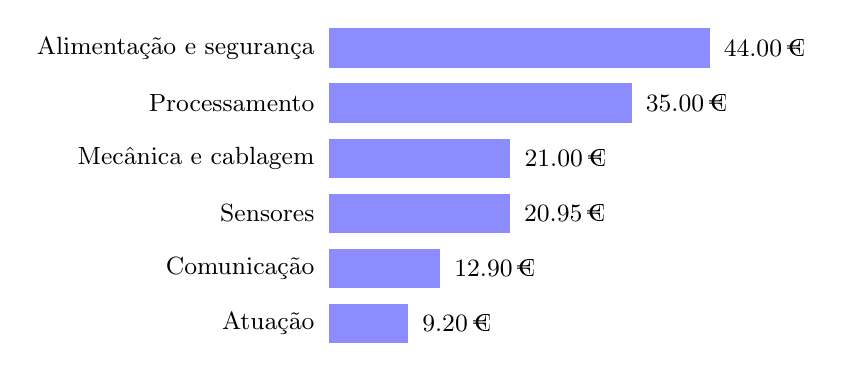
\begin{tikzpicture}[x=0.11cm]
\foreach \lab/\val/\pos in {Alimentação e segurança/44.00/0, Processamento/35.00/1, Mecânica e cablagem/21.00/2, Sensores/20.95/3, Comunicação/12.90/4, Atuação/9.20/5}{
  \node[anchor=east, font=\small] at (0,-\pos*0.7) {\lab};
  \fill[blue!45] (0.5,-\pos*0.7-0.25) rectangle (0.5+\val,-\pos*0.7+0.25);
  \node[anchor=west, font=\small] at (1+\val,-\pos*0.7) {\val\,€};
}
\end{tikzpicture}
\caption{Distribuição do custo do protótipo por grupo.}
\label{fig:custos}
\end{figure}

A alimentação e a segurança representam o maior grupo (cerca de 31\,\% do total), mais do que o processamento. Isto resulta de a bateria e os reguladores terem de ser dimensionados para os picos de corrente dos servos e de se ter incluído desde o início um interruptor de corte dos servos e proteção por fusível. A placa de desenvolvimento é o componente individual mais caro (25\,\%), seguida do GY-85 (15\,\%). Os sensores e os atuadores, que são o núcleo funcional do sistema, custam em conjunto cerca de 21\,\%.

A troca da MPU6050 pelo GY-85 aumentou o custo em cerca de 15~€. Uma segunda \gls{imu} na base, para a compensação antecipativa, acrescentaria outro tanto se fosse também um GY-85 e levaria o total acima dos 150~€; para essa função bastaria um sensor de seis eixos mais barato, já que o magnetómetro não é necessário.

Se o sistema viesse a ser produzido em série, o custo por unidade poderia baixar bastante. A placa NUCLEO seria substituída por uma placa de circuito impresso própria, apenas com o microcontrolador e os componentes necessários, ou por um microcontrolador mais simples, já que o estudo do estado da arte mostrou que um filtro complementar e dois \gls{pid} não exigem um Cortex-M7. Um microcontrolador com Bluetooth integrado, como o ESP32-S3, eliminaria também o módulo de comunicação. Em contrapartida, um produto comercial teria custos que um protótipo não tem, como o projeto da placa, os ensaios de conformidade descritos no capítulo~\ref{ch:seguranca} e a embalagem.

\acompletar{horas de trabalho da equipa, se se pretender incluir o custo de engenharia}

\chapter{Segurança e Conformidade}
\label{ch:seguranca}

Para a análise de segurança considerou-se que a plataforma seria comercializada como um brinquedo educativo, destinado a crianças a partir dos 8 anos, comandado pelo telemóvel. Esta hipótese é a mais exigente, porque os brinquedos têm requisitos próprios de segurança e o utilizador não tem formação técnica. Um protótipo académico, usado apenas em laboratório, não é colocado no mercado e não tem de ostentar a marcação \gls{ce} \cite{blueguide2022}; ainda assim, a análise permitiu incorporar no projeto medidas que um produto certificado teria de ter.

\section{Legislação e normas aplicáveis}
Como brinquedo elétrico com um emissor Bluetooth e uma bateria, o produto ficaria abrangido pelos atos e normas da tabela~\ref{tab:legislacao}.

\begin{table}[H]
\centering\small
\caption{Legislação e normas aplicáveis a um brinquedo com estas características.}
\begin{tabularx}{\textwidth}{>{\raggedright\arraybackslash}p{4.6cm}Y}
\toprule
Legislação ou norma & Âmbito\\\midrule
Diretiva 2009/48/CE \cite{toy2009} & Segurança dos brinquedos; em vigor\\
Regulamento (UE) 2025/2509 \cite{toy2025} & Substitui a diretiva a partir de 1 de agosto de 2030; introduz o passaporte digital do produto e exige avaliar os riscos dos brinquedos ligados digitalmente \cite{eurofinstoy}\\
Diretiva 2014/53/UE (\acrshort{red}) \cite{red2014} & Equipamentos de rádio (Bluetooth)\\
Diretivas 2011/65/UE (\acrshort{rohs}) e 2012/19/UE (\acrshort{reee}) \cite{rohs2011,weee2012} & Substâncias perigosas e fim de vida do equipamento elétrico\\
Regulamento (UE) 2023/1542 \cite{battery2023} & Baterias\\
EN 71-1, EN 71-2 e EN 71-3 \cite{en71} & Propriedades mecânicas e físicas, inflamabilidade e migração de elementos químicos\\
EN IEC 62115 \cite{en62115} & Segurança de brinquedos elétricos\\
EN 300 328, EN 301 489-1 e -17 \cite{en300328,en301489} & Espetro e compatibilidade eletromagnética do rádio\\
\bottomrule
\end{tabularx}
\label{tab:legislacao}
\end{table}

\section{Requisitos para brinquedos e resposta do projeto}
A tabela~\ref{tab:brinquedo} cruza os principais requisitos de segurança dos brinquedos com a situação do protótipo.

\begin{table}[H]
\centering\small
\caption{Requisitos de segurança para brinquedos e situação do protótipo.}
\begin{tabularx}{\textwidth}{>{\raggedright\arraybackslash}p{3.2cm}YY}
\toprule
Requisito & Situação no protótipo & Alteração para um produto\\\midrule
Tensão nominal não superior a \SI{24}{\volt} \cite{toy2009} & Cumpre: máximo de \SI{8.4}{\volt} (RNF12) & --\\
Bateria e eletrónica inacessíveis sem ferramenta & Cumpre: caixa fechada com parafusos (SEG-08) & --\\
Sem arestas vivas nem pontas (EN 71-1) & Peças impressas com arestas por acabar & Arredondar arestas e rever o acabamento\\
Sem pontos de entalamento de dedos (EN 71-1) & Folgas entre quadro, plataforma e torres; servos com binário elevado & Proteger as zonas de rotação, limitar velocidade e binário, manter o interruptor de corte dos servos\\
Temperatura das partes acessíveis (EN IEC 62115) & Servos e reguladores podem aquecer em bloqueio & Medir temperaturas; deteção de bloqueio em software\\
Bateria segura & LiPo sem proteção própria & Usar bateria com circuito de proteção e carregamento integrado, sem intervenção da criança\\
Materiais (EN 71-2, EN 71-3) & PLA sem tintas & Confirmar inflamabilidade e migração de elementos com o fornecedor do material\\
Brinquedo ligado & Recebe apenas ângulos; não recolhe dados pessoais & Ligação protegida por emparelhamento; informação ao utilizador\\
\bottomrule
\end{tabularx}
\label{tab:brinquedo}
\end{table}

O protótipo cumpre os requisitos elétricos de base, mas não está pronto para ser um brinquedo: as maiores lacunas são a bateria LiPo sem proteção e os pontos de entalamento no mecanismo. Ambas têm solução conhecida e baixo custo.

\section{Análise de riscos}
A análise seguiu o método da EN ISO 12100: identificar os perigos, estimar o risco como produto da gravidade (G) pela probabilidade (P), numa escala de 1 a 3, e definir medidas para o reduzir. Considera-se aceitável um risco residual igual ou inferior a 3.

\begin{table}[H]
\centering\scriptsize
\caption{Análise de riscos.}
\begin{tabularx}{\textwidth}{>{\raggedright\arraybackslash}p{2.4cm}ccc>{\raggedright\arraybackslash}Yc}
\toprule
Perigo & G & P & R & Medidas de redução & R res.\\\midrule
Entalamento de dedos & 2 & 2 & 4 & Limites de amplitude e velocidade; proteção das zonas de rotação; interruptor de corte dos servos & 2\\
Movimento inesperado & 2 & 2 & 4 & Arranque desarmado; armar explícito; \textit{watchdog}; modo seguro & 2\\
Incêndio da bateria & 3 & 1 & 3 & Fusível; bateria com proteção; monitorização da tensão & 2\\
Sobreaquecimento dos servos & 1 & 2 & 2 & Limites de comando; deteção de bloqueio & 1\\
Arestas vivas & 1 & 2 & 2 & Acabamento das peças & 1\\
Choque elétrico & 1 & 1 & 1 & Muito baixa tensão & 1\\
\bottomrule
\end{tabularx}
\label{tab:riscos}
\end{table}

\section{Funções de segurança implementadas}
As medidas anteriores traduzem-se nas seguintes funções, verificadas pelos testes T-SEG (capítulo~\ref{ch:testes}):
\begin{itemize}
\item \textbf{Corte dos servos por hardware:} um interruptor de dois polos corta a alimentação dos servos sem depender do microcontrolador.
\item \textbf{Arranque seguro:} o sistema arranca desarmado e só se move depois de calibrado e armado.
\item \textbf{Modo seguro:} sem referências válidas durante \SI{1}{\second}, ou com bateria baixa, a plataforma volta suavemente à horizontal.
\item \textbf{Limites em software:} amplitude, velocidade e largura de impulso dos servos limitadas.
\item \textbf{\textit{Watchdog}:} reinício automático em caso de bloqueio do programa.
\item \textbf{Proteção elétrica:} fusível, interruptor geral e eletrónica fechada numa caixa aparafusada.
\end{itemize}

%\chapter{Conclusões e Trabalho Futuro}
\label{ch:conclusao}

\section{Conclusões}
Este trabalho tem como objetivo o desenvolvimento de uma plataforma estabilizada de dois eixos, capaz de acompanhar a inclinação de um telemóvel e de se manter nivelada perante perturbações da base.

O estudo do estado da arte mostrou que este tipo de sistema pode ser construído com componentes de baixo custo. Os trabalhos analisados indicam que uma \gls{imu} associada a um filtro de fusão simples permite obter uma estimativa da atitude adequada ao controlo e que um controlador \gls{pid} é, em muitos casos, suficiente para estabilizar plataformas pequenas. Os métodos mais avançados trazem vantagens sobretudo quando existe um modelo fiável do sistema e acesso à velocidade ou à corrente dos atuadores, o que não acontece com servos de modelismo.

O paralelismo com os drones mostrou que o problema da plataforma é, em grande parte, um subconjunto do controlo de atitude de um multirrotor. A separação entre estimação e controlo, a limitação do termo integral, o \textit{failsafe} perante perda de ligação e o passo de armar antes de mover os atuadores foram transpostos diretamente para a arquitetura proposta.

A estrutura mecânica, modelada em OpenSCAD, é um \textit{gimbal} em série com os dois eixos a cruzarem-se no mesmo ponto, o que elimina o acoplamento mecânico entre eixos e simplifica a calibração dos servos. O hardware assenta numa NUCLEO-F767ZI, numa \gls{imu} GY-85, em dois servos MG996R e num módulo Bluetooth de modo duplo, com alimentação por bateria e regulação separada para os servos e para a eletrónica. O esquema elétrico e a atribuição de pinos ficaram definidos. O dimensionamento mostrou que o regulador dos servos tem de suportar os picos de corrente em bloqueio e que a autonomia estimada excede largamente o requisito. O software foi organizado em camadas e módulos com interfaces bem definidas, o que permitiu, por exemplo, trocar de sensor alterando apenas o respetivo \textit{driver}; para cada módulo foram definidos procedimentos e vetores de teste ligados aos requisitos.

O custo estimado do protótipo é de cerca de 143~€, dentro do limite definido. A análise de segurança, feita considerando o equipamento como um brinquedo, mostrou que o protótipo cumpre os requisitos elétricos de base, como a tensão máxima e a inacessibilidade da eletrónica, mas que um produto comercial teria de proteger os pontos de entalamento e usar uma bateria com proteção própria.

\section{Trabalho futuro}
Os próximos passos do trabalho são os seguintes:
\begin{itemize}
\item implementar e testar cada módulo de acordo com o capítulo~\ref{ch:testes};
\item calibrar os servos e identificar a dinâmica do conjunto servo--plataforma;
\item desenvolver a aplicação do telemóvel;
\item afinar os controladores e comparar o \gls{pid} com e sem compensação antecipativa;
\item avaliar a utilidade de uma segunda \gls{imu} na base e de algoritmos de fusão mais completos;
\item rever estas conclusões à luz dos resultados experimentais.
\end{itemize}

\acompletar{rever as conclusões quando houver resultados}

%\include{chapters/chapter3}	% Uncomment the lines as you write the chapters,
								% where 'chapter3' refers to a file chapter3.tex
%...							% in the 'chapters' folder
								

%%%%%%%%%%%%%%%%%%%%%%%%%%%%%%%%%%%%%%%%%%%%%%%%%%%%%%%%%%%%%%%%%%%%%%%%%%%%%%%%%%%%%%%%%
% Print the bibliographic references using the ieeetr format from the 'sampleRefs.bib' file (root folder)

\cleardoublepage
\printrefereces{referencias}		% Change the 'sampleRefs' name to match your .bib file name,
								% a good option to make bib files is https://www.jabref.org/
%%%%%%%%%%%%%%%%%%%%%%%%%%%%%%%%%%%%%%%%%%%%%%%%%%%%%%%%%%%%%%%%%%%%%%%%%%%%%%%%%%%%%%%%%
%\begin{appendices}
% Include the appendices of the dissertation as separate files from the 'chapters' folder

%\include{chapters/appendixA}	% Uncomment the lines as you write the appendices,
%\include{chapters/appendixB}	% or comment the lines if not used

%\end{appendices}
%%%%%%%%%%%%%%%%%%%%%%%%%%%%%%%%%%%%%%%%%%%%%%%%%%%%%%%%%%%%%%%%%%%%%%%%%%%%%%%%%%%%%%%%%
\end{document}  
